% Principal Anteproy

% header
\documentclass[12pt, titlepage,oneside]{article}
% ******** vmargin settings *********
\usepackage{vmargin} %This give you full control over the used page area, it maybe not the idea od Latex to do so, but I wanted to reduce to amount of white space on the page
%\setcitestyle{round,authoryear,citesep={;}, aysep={,}}
\setpapersize{USletter}
\setmarginsrb{4cm}%			%linker Rand, left edge --- izquierda
{2cm}%     %oberer Rand, top edge  --- arriba
{3cm}%		% -- derecha
{2cm}%   % -- abajo
{12pt}%			%Kopfzeilenhöhe, header hight
{1cm}%   	  %Kopfzeilenabstand, header distance
{12pt}%				%Fußzeilenhoehe footer hight
{1cm}%    	  %Fusszeilenabstand, footer distance   
% ********* Lenguage definition *******

\usepackage[spanish]{layout}
\usepackage[spanish,activeacute]{babel}
\usepackage[utf8]{inputenc}
\usepackage{hyperref}
\usepackage{enumerate}
\usepackage{amsmath}
\usepackage{amsfonts}
\usepackage{amssymb}
\usepackage{fancyhdr}
\usepackage{bbm}
\usepackage{tocloft}
\usepackage{array}
\usepackage{titlesec}
\usepackage{booktabs}
\usepackage[flushleft]{threeparttable}

\usepackage{makeidx}
\usepackage{lmodern}
\usepackage{kpfonts}
\usepackage{multirow}
\usepackage{booktabs}
% ********* Graphics definition *******
%\usepackage [dvips]             {graphicx}
%\usepackage{colortbl}
\usepackage[pdftex]{graphicx} % required to import graphic files
\usepackage{color} 	  % allows to mark some entries in the tables with color
\usepackage{eso-pic}  % these two are required to add the little picture on top of every page
\usepackage{everyshi} % these two are required to add the little picture on top of every page
\usepackage{apacite}
%\usepackage[left=2cm,right=2cm,top=2cm,bottom=2cm]{geometry}
\usepackage[numbers]{natbib}
\bibliographystyle{IEEEtranN}

% ******************* Entornos adicionales. ********************************
\setcounter{secnumdepth}{4}
\setcounter{tocdepth}{4}
\titleformat{\paragraph}
{\normalfont\normalsize\bfseries}{\theparagraph}{1em}{}
\titlespacing*{\paragraph}
{0pt}{3.25ex plus 1ex minus .2ex}{1.5ex plus .2ex}

\newtheorem{teo}{Teorema}
\newtheorem{defi}{Definici\'on}
\newtheorem{rem}{Remarque}
\newtheorem{col}{Coloquial}
\newtheorem{notacion}{Notaci\'on\'}
\newtheorem{eje}{Ejemplo}
\newtheorem{hip}{Hip\'otesis}
\newcommand{\bh}{\begin{hip}}
\newcommand{\eh}{\end{hip}}

\renewcommand{\contentsname}{Tabla de Contenido}
\renewcommand{\listtablename}{Lista de Tablas}
\renewcommand{\listfigurename}{Lista de Figuras}
\renewcommand{\refname}{REFERENCIAS}
\renewcommand{\tablename}{Tabla}
\renewcommand{\figurename}{Figura}
\renewcommand{\cfttabfont}{Tabla }
\renewcommand{\cftfigfont}{Figura }

\newcolumntype{C}[1]{>{\centering\let\newline\\\arraybackslash\hspace{0pt}}m{#1}} %Para centrar y ajustar tamaño de la columna de una tabla
\newcolumntype{L}[1]{>{\raggedright\let\newline\\\arraybackslash\hspace{0pt}}m{#1}} %Para alinear a la derecha y ajustar tamaño de la columna de una tabla
\newcolumntype{R}[1]{>{\raggedleft\let\newline\\\arraybackslash\hspace{0pt}}m{#1}}%Para alinear a la izquierda y ajustar tamaño de la columna de una tabla
\newcolumntype{M}{>{$\vcenter\bgroup\hbox\bgroup}c<{\egroup\egroup$}} %Para centrar verticalmente el contenido de una celda de una tabla
\typeout{Copyright Alejandro Gil Caicedo} % No cambiar esta linea-

\hyphenation{po-si-bles
al-can-za-bles al-can-za-bi-li-dad lo-cal-ment-te a-que-llas
re-pre-sen-ta-cio-nes cons-tan-te ins-tan-te mo-de-lo es-ta-dos
con-tro-la-ble con-tro-la-bi-li-dad de-sa-rro-llar-se re-fe-ren-cias
Co-lo-ra-do co-rri-en-te re-fe-ren-cia}

\fancyhf{}
\renewcommand{\headrulewidth}{0.5pt}
\renewcommand{\footrulewidth}{0.5pt}
%\setlength{\topmargin}{2.5 cm}
%\setlength{\headheight}{0.7 cm}
%\setlength{\headsep}{1 cm}
%\setlength{\textheight}{19 cm}
%\setlength{\oddsidemargin}{0.5 cm}
%\setlength{\footskip}{0.85 cm}
%\setlength{\textwidth}{16 cm}
%\fancyhead[LE,RO]{\bfseries\thepage}
\fancyhead[L]{\footnotesize\bfseries Implementacion de un manejador de recursos con inteligencia ambiental para una ...}
%\fancyhead[R]{\bfseries\leftmark}
%\frontmatter
%\fancyhead[R]{\footnotesize \bfseries Doctorado en Ingeniería, Pag.\thepage}
%\fancyhead[R]{\footnotesize\bfseries Énfasis en Automática, Pag.\thepage}
%\fancyhead[R]{\footnotesize\bfseries Énfasis en Eléctrica, Pag.\thepage}
%\fancyhead[R]{\footnotesize\bfseries Énfasis en Electrónica, Pag.\thepage}
\fancyhead[R]{\footnotesize\bfseries Pag. \thepage}
%\fancyfoot[L]{\footnotesize\textbf{Nombre del Autor}}

\fancyfoot[R]{\footnotesize\textbf{Propuesta de Trabajo de Grado}}
%\fancyfoot[R]{\footnotesize\textbf{Propuesta de Tesis - Doctorado-.}}

%este es de configuracion de la typografia general

\usepackage[table,xcdraw]{xcolor} %este es una libreria para tablas bonitas
\usepackage{longtable}%este es necesario cuando se tienen tablas grandes
\usepackage{booktabs} %este es necesario para usar el exel2latex 

\usepackage[utf8]{inputenc}%este es para poder tener tildes de una
\usepackage{hyperref}
\usepackage{graphicx}%libreria para insertar imagenes
\hfuzz=.7pt %this one is used to ignore the half letther spceson paragraph problems

%to remoove the default tittle of the bibliograpy import:
\renewcommand{\bibname}{}



\begin{document}
\pagestyle{empty}

%Portada 
\pagestyle{empty}
\begin{center}

\begin{figure}[htbp]
	\centering
		
\includegraphics[width=2cm]{figuras/uv_logo.png}
	\label{Logo_UV}
\end{figure}

\vspace{2cm}

\textbf{\large{IMPLEMENTACI\'ON DE UN MANEJADOR DE RECURSOS CON INTELIGENCIA AMBIENTAL PARA UNA VIVIENDA DEL SOLAR DECATHLON LATIN AMERICA 2019}}

\vspace{4cm}

\large{
JUAN DAVID RAMÍREZ VILLEGAS
}

\vspace{4cm}

\large{UNIVERSIDAD DEL VALLE}\\
\large{FACULTAD DE INGENIERÍA}\\
\large{ESCUELA DE INGENIERÍA ELÉCTRICA Y ELECTRÓNICA}\\
\large{PROGRAMA ACADÉMICO DE INGENIERÍA ELECTRÓNICA}\\
\large{\Today}

%\large {Estudiante: Ing. Andrés Fernando Restrepo Álvarez\\ Director: M.Sc. Carlos Rafael Pinedo.\\ Director: Dr.Ing. Edinson Franco Mejía.}

\vspace{4cm}

\end{center}
\newpage
%Contraportada papu
\pagestyle{empty}
\begin{center}

\begin{figure}[htbp]
	\centering
		
\includegraphics[width=2cm]{figuras/uv_logo.png}
\end{figure}

\vspace{2cm}

\textbf{\large{IMPLEMENTACI\'ON DE UN MANEJADOR DE RECURSOS CON INTELIGENCIA AMBIENTAL PARA UNA VIVIENDA DEL SOLAR DECATHLON LATIN AMERICA 2019}}

\vspace{2cm}

\large{
JUAN DAVID RAMÍREZ VILLEGAS\\
CODIGO: 1427249
}

\vspace{3cm}

\large{ÉDINSON FRANCO MEJÍA, Dr.-Ing.}\\
\large{FABIO GERMÁN GUERRERO, M.Sc.}\\

\vspace{2cm}

\large{UNIVERSIDAD DEL VALLE}\\
\large{FACULTAD DE INGENIERÍA}\\
\large{ESCUELA DE INGENIERÍA ELÉCTRICA Y ELECTRÓNICA}\\
\large{PROGRAMA ACADÉMICO DE INGENIERÍA ELECTRÓNICA}\\
\vspace{1cm}
\large{\Today}

%\large {Estudiante: Ing. Andrés Fernando Restrepo Álvarez\\ Director: M.Sc. Carlos Rafael Pinedo.\\ Director: Dr.Ing. Edinson Franco Mejía.}

\vspace{4cm}

\end{center}
\newpage

\renewcommand{\thepage}{\roman{page}} \setcounter{page}{2}%pongo la enumeracion romana en 2
\tocloftpagestyle{fancy} %Estilo de la pagina de la table de contenido
\tableofcontents %pongo tabla de ocntenido
\newpage

\listoffigures %en otra pagina pongo las dos tablas restantes
\listoftables
\newpage

\renewcommand{\thepage}{\arabic{page}} \setcounter{page}{4}
\pagestyle{fancy}%estilo de los demas apartados:

\customsection{Introducción}
\subsection{Contexto introductorio}
No es para nadie una sorpresa que durante este siglo, las nuevas generaciones que nacen rodeadas de la tecnología y están cambiando las costumbres y el paradigma actual de lo que significa una vivienda, con una sociedad cada vez más relacionada con la tecnología, nuevos desafíos de diseño e implementación se plantean para satisfacer las expectativas de las nuevas generaciones.
\vspace{0.5cm}\\
Básicamente el más importante beneficio utilizar la tecnología en viviendas comerciales es el proveer de servicios y facilidades a personas discapacitadas y ancianos \cite{GiralSala2016}, por otra parte, tenemos beneficios de monitorización y la capacidad de añadir herramientas que permitan la integración con redes eléctricas inteligentes. La popularidad de sistemas inteligentes ha venido incrementando debido al confort adicional, y herramientas de seguridad que pueden recibir los usuarios. 
\vspace{0.5cm}\\
Por lo tanto, hay ciertos factores que deben ser tenidos en cuenta a la hora de diseñar un sistema de control y monitoreo de la vivienda, en este documento se explicará el proceso de diseño e implementación de un software para el manejo inteligente de una vivienda del Solar Decathlon Latinoamérica utilizando diferentes tecnologías de \textit{frontend} y \textit{backend}
\vspace{0.5cm}\\
La arquitectura desarrollada se puede describir en 3 productos:
 
\begin{enumerate}
	\item Un servicio de \textit{backend} serverless basado en: un broker de Mqtt, un servicio de almacenamiento de datos tipo S3, una base de datos relacional tipo MySql e interfaces http basadas en funciones de nube. 
	\item Un programa encargado de administrar y controlar todas las rutinas de comunicación, reporte y almacenamiento en el sitio de control con su respectiva interfaz de usuario.
	\item Una aplicación celular capaz de monitorear y controlar los datos generados localmente y los actuadores de la vivienda del Solar Decathlon.
\end{enumerate}


%\subsection{Planteamiento del problema}

Hoy en día las tecnologías orientadas internet y la mayoría de los objetos utilizados en la cotidianidad, en general, están cada vez más relacionadas entre sí; el pasado año se vio un incremento de 2.79 billones de nuevos dispositivos conectados a la red de redes (entre los cuales no solo se encuentran celulares computadores y tablets). Nuevos dispositivos como aires acondicionados, televisores y electrodomésticos en general son lanzados al mercado con la capacidad de comunicarse con el usuario a través de aplicaciones web o dispositivos móviles día tras día. Lo anterior se debe al aumento en los desarrollos de hardware y software para sistemas con la capacidad de acceso a la red; es decir, con la capacidad de acceder a comunicaciones inalámbricas, servidores locales, servicios en la nube, entre otras propuestas.
\vspace{0.5cm}\\
Teniendo en cuenta lo anterior, muchos sistemas basados en diseños embebidos y/o tarjetas de desarrollo CPU se han propuesto como forma de integración y aplicación de sistemas de domótica en el hogar. La mayoría de estos proyectos o aplicativos son pensados para automatizar tareas específicas o agregarle una componente de comunicación remota al hogar. Si bien estos son puntos atractivos para un consumidor, el concepto de vivienda inteligente se puede expandir por más terrenos, tan diversos como el que se presentará en este documento.
\vspace{0.5cm}\\
Un concepto tan abierto y ventajoso como el de la vivienda inteligente o el internet de las cosas puede ser utilizado en el marco del concurso Solar Decatlón Latín América, el cual plantea el desarrollo de un proyecto de vivienda residencial amigable con el medio ambiente, donde el diseño arquitectónico ganador se decide en base a 10 indicadores cada uno con 100 puntos calificados de manera cualitativa y cuantitativa por los jueces.
\vspace{0.5cm}\\
Para la porción de la puntuación que es calificada de manera cuantitativa los jueces utilizan medidores que, dependiendo del indicador, puede corresponder para monitorear o medir el consumo eléctrico, temperatura, humedad, picos de consumo (3 kilo watts) donde se establece un valor de mínimo y máximo para un rango de puntos desde cero hasta la máxima calificación.
\vspace{0.5cm}\\
Considerando lo anterior, se plantea realizar la mejor aproximación tecnológica para cumplir de manera más acercada los indicadores de: eficiencia energética, innovación, balance eléctrico energético y condiciones de confort, puesto que son aquellos que pueden ser solucionados gestionados y monitoreados por tecnologías actuales. Basándose en lo expuesto anteriormente se plantea la siguiente pregunta al problema de ingeniería:
\vspace{0.5cm}\\
¿Cómo diseñar e implementar un sistema software que permita la gestión de cargas eléctricas y el monitoreo de variables físicas de manera local y remota para el concurso del Solar Decatlón latín América?.
%\subsection{Justificación}
Respecto a la vivienda inteligente o la domótica en el hogar, se puede decir que la literatura es amplia y que existen diferentes propuestas comerciales de desarrollo como lo son: Calaos, Domoticz, Home Assistant, OpenHAB, OpenMotics, donde cada marca propone su marco de trabajo, y diferentes plataformas de desarrollo tanto software como hardware. Una desventaja de estas propuestas es su interfaz hardware, en la mayoría de los casos el hardware adicional corresponde a dispositivos desarrollados y mantenidos por ellos mismos, lo que significa que limita la escalabilidad de las
\vspace{0.5cm}\\
Las anteriores tecnologías son propuestas donde un centro de mando controla dispositivos externos, pero, por otra parte, si pensamos en cada módulo hardware con la capacidad de conectarse a la red de redes de manera independiente (Iot) como lo hace la propuesta realizada el en proyecto del “Smart switch” \cite{GiralSala2016}; se tiene como ventaja la independencia sobre las características físicas del hogar o de la capacitación técnica del instalador del sistema, pero como desventaja, al momento de escalar el problema a un mayor número de circuitos se pueden presentar problemas de saturación de la red inalámbrica (wifi) y sería más costoso debido al hardware adicional para cada nuevo circuito que se desee controlar.
\vspace{0.5cm}\\
Teniendo en cuenta las comparaciones anteriores, se podría pensar que un sistema que englobe varios sub sistemas podría ser el adecuado desde el punto de vista de la escalabilidad, pero esa no es la única razón; Hoy en día los métodos de generación alternativa y energía renovable se encuentran en crecimiento, por lo que nace la necesidad de interconectar redes eléctricas inteligentes, es decir, una red con un componente de generación y consumo tanto como AC y DC. Este tipo de topología eléctrica se le conoce como nanogrid, y se ampliará la teoría respecto a este concepto en futuras secciones del documento. Esta topología eléctrica añade como variable la generación eléctrica junto con una nueva forma fisica de energía (corriente directa).
\vspace{0.5cm}\\
Inclusive, se puede observar que artículos académicos se han dedicado a analizar este concepto en el contexto Colombiano,  por ejemplo un estudio sobre microgrids mencionó la importancia y necesidad de implementar viviendas inteligentes como se ve a continuación: “desde el contexto de seguridad eléctrica, equidad social y mitigación del impacto ambiental en Colombia, el sistema energético debe afrontar los nuevos retos requeridos para satisfacer la demanda. Desde un punto de vista técnico, es necesario dotar la red tradicional con las características de una red inteligente ”. 
\vspace{0.5cm}\\
Pero ¿acaso una red inteligente implica una casa inteligente? La respuesta es; parcialmente sí. Considerando que hoy en día toda vivienda realiza un monitoreo o medición de al menos 2 variables críticas; el consumo eléctrico, y el consumo de agua, ambos son de interés para la compañía prestadora de servicios públicos en la vivienda.
\vspace{0.5cm}\\
Resaltando la importancia de las anteriores variables físicas y teniendo en cuenta el modelo de nanogrid al cual podría llegar a ser una vivienda; la gestion de informacion adicional a la necesaria para cumplir la domótica resalta al a vista. En adición, estos componentes de generación y consumo eléctrico son la base para hablar sobre el impacto ambiental de las costumbres internas de los habitantes de un hogar, que resulta de vital interés para la optimización de los 4 ítems de calificación en el solar decathlon.
\vspace{0.5cm}\\
Finalizando, una propuesta integral de domótica y gestión inteligente de información como la que se presenta en este documento facilita la verificación y el cumplimiento de los ítems anteriormente mencionados, contemplando que el sistema quedara diseñado de tal manera que sea fácil la escalabilidad para aspectos como; seguridad, aseguramiento contra accidentes (incendio), viviendas de diferente tamaño, interfaz de voz y video.


%\subsection{Objetivos}

\subsubsection{Objetivo general}
Implementar un sistema software para una vivienda del Solar Decathlon capaz de gestionar el control y la medición de variables físicas de manera local y remota.
\subsubsection{Objetivos especificos}
\begin{itemize}
	\item Diseñar una API que permita implementar interfaces gráficas, haciendo uso de imágenes personalizadas, para lograr una interacción amigable con el usuario.
	\item Implementar una aplicación software que funcione en el sitio y le permita al usuario gestionar la información de interés y controlar las cargas eléctricas.
	\item Implementar un aplicativo móvil que le permita al usuario tener la experiencia de interactuar con una vivienda inteligente.
\end{itemize}


\subsection{Lineamientos de desarrollo}
Debido a la naturaleza del proyecto, parte de los aspectos definidos al momento de establecer el anteproyecto fueron unas necesidades funcionales explicadas en el formato \ref{tab0}.

% Please add the following required packages to your document preamble:
% \usepackage[table,xcdraw]{xcolor}
% If you use beamer only pass "xcolor=table" option, i.e. \documentclass[xcolor=table]{beamer}

\begin{longtable}[c]{lllc}
\hline
\multicolumn{1}{|l|}{
\begin{tabular}[c]{@{}l@{}}
	
\includegraphics[width=1cm]{figuras/uv_logo.png}
\end{tabular}
} 
& 
\multicolumn{2}{l|}{\cellcolor[HTML]{808080}{\color[HTML]{FFFFFF} \textbf{
\begin{tabular}[c]{@{}l@{}}Universidad del Valle\\--Implementación de un gestionado de recursos\\ para el hogar con inteligencia ambiental. ---\end{tabular}}}}
&
\multicolumn{1}{c|}{\textbf{\begin{tabular}[c]{@{}c@{}}Rev:\\ 003\end{tabular}}} \\ \hline
\endfirsthead
%
\endhead
%
\multicolumn{2}{|l|}{\textbf{\begin{tabular}[c]{@{}l@{}}Título:\\   ESPECIFICACIÓN DE \\ REQUERIMIENTOS \\ FUNCIONALES\end{tabular}}} & \multicolumn{1}{l|}{\textbf{\begin{tabular}[c]{@{}l@{}}Documento :\\ ERF-000\end{tabular}}} & \multicolumn{1}{c|}{\textbf{\begin{tabular}[c]{@{}c@{}}Página :\\ 1 de 1\end{tabular}}} \\ \hline
 &  &  & \multicolumn{1}{l}{} \\ \hline
\rowcolor[HTML]{808080} 
\multicolumn{4}{|c|}{\cellcolor[HTML]{808080}\textbf{REVISIÓN HISTÓRICA}} \\ \hline
\rowcolor[HTML]{808080} 
\multicolumn{1}{|l|}{\cellcolor[HTML]{808080}\textbf{Rev.}} & \multicolumn{1}{l|}{\cellcolor[HTML]{808080}\textbf{Descripción del Cambio}} & \multicolumn{1}{l|}{\cellcolor[HTML]{808080}\textbf{Autor}} & \multicolumn{1}{l|}{\cellcolor[HTML]{808080}\textbf{Fecha}} \\ \hline
\multicolumn{1}{|l|}{001} & \multicolumn{1}{l|}{Construcción del documento} & \multicolumn{1}{l|}{\begin{tabular}[c]{@{}l@{}}Juan David Ramirez\\ Villegas\end{tabular}} & \multicolumn{1}{l|}{18/03/2017} \\ \hline
\multicolumn{1}{|l|}{002} & \multicolumn{1}{l|}{Correcciones} & \multicolumn{1}{l|}{\begin{tabular}[c]{@{}l@{}}Juan David Ramírez\\ Villegas\end{tabular}} & \multicolumn{1}{l|}{15/11/2017} \\ \hline
\multicolumn{1}{|l|}{003} & \multicolumn{1}{l|}{Revisión} & \multicolumn{1}{l|}{\begin{tabular}[c]{@{}l@{}}Juan David Ramírez\\ Villegas\end{tabular}} & \multicolumn{1}{l|}{18/12/2017} \\ \hline
 &  &  & \multicolumn{1}{l}{} \\ \hline
\rowcolor[HTML]{808080} 
\multicolumn{1}{|l|}{\cellcolor[HTML]{808080}\textbf{Ref \#}} & \multicolumn{2}{l|}{\cellcolor[HTML]{808080}\textbf{Funciones}} & \multicolumn{1}{l|}{\cellcolor[HTML]{808080}\textbf{Categoría}} \\ \hline
\multicolumn{1}{|l|}{1.0} & \multicolumn{2}{l|}{USER APP (application móvil)} & \multicolumn{1}{c|}{\textbf{O}} \\ \hline
\multicolumn{1}{|l|}{1.1} & \multicolumn{2}{l|}{\begin{tabular}[c]{@{}l@{}}El usuario debe poder acceder a la \\ información medida en tiempo real.\end{tabular}} & \multicolumn{1}{c|}{\textbf{E}} \\ \hline
\multicolumn{1}{|l|}{1.2} & \multicolumn{2}{l|}{\begin{tabular}[c]{@{}l@{}}El usuario debe poder acceder a los datos \\ históricos recopilados en el mes y la \\ relación de sus gastos con ellos.\end{tabular}} & \multicolumn{1}{c|}{\textbf{O}} \\ \hline
\multicolumn{1}{|l|}{1.3} & \multicolumn{2}{l|}{\begin{tabular}[c]{@{}l@{}}El usuario debe poder cambiar los \\ parámetros de configuración escogidos\\  por defecto para la vivienda del\\  Solar Decathlon.\end{tabular}} & \multicolumn{1}{c|}{\textbf{E}} \\ \hline
\multicolumn{1}{|l|}{1.4} & \multicolumn{2}{l|}{\begin{tabular}[c]{@{}l@{}}El usuario debe recibir recomendaciones\\  para mejorar su entorno y su huella \\ hídrica cada cierto tiempo.\end{tabular}} & \multicolumn{1}{c|}{\textbf{E}} \\ \hline
\multicolumn{1}{|l|}{1.5} & \multicolumn{2}{l|}{\begin{tabular}[c]{@{}l@{}}La aplicación notificará al usuario\\ cuando la factura de energía o agua\\  esté vencida.\end{tabular}} & \multicolumn{1}{c|}{\textbf{O}} \\ \hline
\multicolumn{1}{|l|}{1.6} & \multicolumn{2}{l|}{\begin{tabular}[c]{@{}l@{}}El usuario debe ser capaz de ver un \\ índice del impacto ambiental de su\\  estilo de vida basado en datos \\ cualitativos y cuantitativos\end{tabular}} & \multicolumn{1}{c|}{\textbf{E}} \\ \hline
\multicolumn{1}{|l|}{1.7} & \multicolumn{2}{l|}{\begin{tabular}[c]{@{}l@{}}El sistema debe ser capaz de notificar \\ las pérdidas eléctricas, y por consiguiente\\  económicas, de un mal uso de los horarios\\  establecidos por defecto.\end{tabular}} & \multicolumn{1}{c|}{\textbf{O}} \\ \hline
\multicolumn{1}{|l|}{2.0} & \multicolumn{2}{l|}{HOUSE MANAGER (Aplicación en sitio)} & \multicolumn{1}{c|}{\textbf{E}} \\ \hline
\multicolumn{1}{|l|}{2.1} & \multicolumn{2}{l|}{\begin{tabular}[c]{@{}l@{}}El sistema debe mostrar gráficamente \\ la cantidad de agua y potencia consumida\\  durante el día contrastándolas con un \\ valor máximo recomendado.\end{tabular}} & \multicolumn{1}{c|}{\textbf{E}} \\ \hline
\multicolumn{1}{|l|}{2.2} & \multicolumn{2}{l|}{\begin{tabular}[c]{@{}l@{}}Por defecto, el uso de las cargas \\ eléctricas más significativas debe\\  programarse durante los picos de \\ generación en la casa. Estos horarios \\ podrán ser modificados bajo una \\ advertencia de uso no eficiente.\end{tabular}} & \multicolumn{1}{c|}{\textbf{E}} \\ \hline
\multicolumn{1}{|l|}{2.3} & \multicolumn{2}{l|}{\begin{tabular}[c]{@{}l@{}}El usuario debe poder acceder \\ a la información medida en tiempo real.\end{tabular}} & \multicolumn{1}{c|}{\textbf{E}} \\ \hline
\multicolumn{1}{|l|}{2.4} & \multicolumn{2}{l|}{\begin{tabular}[c]{@{}l@{}}El sistema debe poder comunicarse \\ con una base de datos que represente \\ todas las variables y el estado de los \\ circuitos de la vivienda.\end{tabular}} & \multicolumn{1}{c|}{\textbf{E}} \\ \hline
\caption{Requerimientos Funcionales del sistema}
\label{tab0}\\
\end{longtable}
La columna de la categoría indica si el requerimiento indicado es uno esencial (E) u opcional (O) para el desarrollo del sistema. Este documento será de gran importancia puesto que definió los lineamientos de desarrollo de todas las aplicaciones.



\section{Marco Teorico}

Para la optima comprension del proyecto de ingenieria explicado en este documento es necesario el entendimiento de diferentes conceptos, tecnologias o teorias. Estos conceptos seran explicados de manera breve en el transcurso de este capitulo, 

\subsection{Arquitectura.}
Se define como un conjunto de componentes de software que operan en de manera relacionada y utilizan interfaces entre ellos. Los componentes de software utilizan un conjunto de herramientas de programación como APIs, Bibliotecas, Frameworks, para su óptimo diseño. Como aclaración las herramientas mencionadas anteriormente se definen como:

\begin{itemize}
	\item \textbf{API (Application Programming Interface):} Es un conjunto de subrutinas, funciones y procedimientos (o métodos, en la programación orientada a objetos) que ofrece cierta biblioteca para ser utilizado por otro software como una capa de abstracción.
    
	\item \textbf{Framework:} En el marco de desarrollo de software, un Framework (entorno de trabajo) corresponde a la estructura  modular que sirve de base para la organización y desarrollo de software. Normalmente, pueden incluir soporte para lenguajes de programación, librerías, entre otras. 
	\item \textbf{Biblioteca:} En programación, una biblioteca o librería es un conjunto de implementaciones funcionales, diseñadas en un lenguaje de programación específico, la cual ofrece una interfaz para la funcionalidad que se invoca.
\end{itemize}

La arquitectura de software que se implementó en este proyecto consta de 3 bloques importantes; un servicio en la nube, una aplicacion celular y una aplicacion de escrtorio. Estos a su vez utilizan herramientas, como las anteriormente descritas, para comunicar o relacionar elementos internamente.


\subsection{Programacion orientada a objetos}

**** describir muy bien la iteraccion shild parent en este paradigma de desarrollo puesto que se menciona mucho en el documento

\subsection{Servidor}

Un módulo hardware y software con amplia capacidad de almacenamiento y procesamiento. Desde el punto de vista del software, los servidores son programas de computador que atienden las peticiones de otros programas llamados clientes. Dentro de estos llamados los principales servicios de un servidor son: compartir datos, información y recursos de hardware. Desde el punto de vista de hardware toda la información entrante de los dispositivos (clientes) es recibida a través de una interfaz de red y reconocida para su posterior procesamiento y almacenamiento.
Desde una perspectiva mas simplista un servidor es un computador con especificaciones de hardware fijas como: ram, cpu, memoria intena, etc, enfocado unicamente en ofrecer los servicios anteriormente mencionados.


\subsection{TCP y TLS}

** hablar del metodo de comunicacion sencillo de tcp (asegurar la recepcion) y su version encriptada Tls

\subsection{JWT}

*** explicar el funcionamiento del estandar de los json web token y los diferentes metodos de encriptacion.

\subsection{Mqtt}

*****Definir de manegra generalizada el protocolo mqtt

\subsection{Http}

*****Definir de manegra generalizada el protocolo http


\subsection{Serverless}

**hablar del concepto de serverless teniendo en cuenta que ya se explico el conepto tradicional de servidor

\subsection{Backend}

****misma historia para el backend dado que ya se hablo del servidor en su generalidad


\subsection{Aplicación web.}

Una aplicación web es un programa que se codifica en un lenguaje interpretable por los navegadores web, esto le permite a la aplicacion ser independiente del sistema operativo y depender de interpretador web (navegador). Dentro de los lenguajes utilizados como desarrollo para aplicaciones web se tienen: html, javascript, php, asp, python, ruby, etc. 

\subsection{Aplicación de escritorio.} 

Una aplicacion escritorio es cualquier software que pueda ser instalado en un computador o sistema de cómputo, y que permita ejecutar ciertas rutinas. En este sentido una aplicación web puede ser una aplicación de escritorio. Los lenguajes de programación de aplicaciones de escritorio son un conjunto más amplio, los que más predominan son aquellos basados en máquinas virtuales o entornos de ejecución puesto que permiten realizar desarrollos independientes del sistema operativo. Dentro de los más conocidos están los lenguajes: Java, Python, C++, Golang, etc.
\vspace{0.5cm}\\
Dentro de los elementos materiales del sistema se encuentran los dispositivos que van a encargarse de la capa física durante el proceso de comunicación y adquisición de datos, a continuación se definirán los componentes más importantes de estos componentes.

\subsection{Frontend}

** describir el concepto de frontend teniendo en cuenta los dos conceptos anteriormente pencionados 

\subsection{Dispositivo}
Un dispositivo es objeto hardware que puede ser visto como un sistema embebido con capacidades de procesamiento y comunicación a diferentes redes. En el dispositivo hardware reside el software que sirve como el manejador de las magnitudes físicas, voltajes, o sensores que están conectadas a él. Este componente normalmente posee las herramientas para el envío de información a servidores locales o remotos, en adición, dentro de los componentes que integran un dispositivo se tienen los siguientes:

\begin{itemize}
	\item \textbf{Sistema de archivos:} Este componente de software es el encargado de almacenar los datos del sistema ya sea localmente, en un servidor de manera remota. Además de lo anterior, este módulo sirve para el almacenamiento de la información necesaria para el funcionamiento del sistema operativo. 
    
	\item \textbf{Colector Cliente:} Este componente es el encargado de gestionar toda la información de los sensores que será enviada a manera de flujos de datos utilizando un protocolo de comunicación, esta capa de software añade los campos de metadata (control y gestión) para la efectiva comunicación.
	\item \textbf{Capa de Sensores:} Este software es el encargado de proveer todos los drivers lógicos para la coneccion de los elementos físicos conectados al dispositivo.
\end{itemize}

Debido al tiempo estipulado para el proyecto el dispositivo y los métodos de adquisición no serán de alta importancia en el desarrollo de la arquitectura y se asumirá que todo desarrollo de los dispositivos debe tener solucionada la comunicación con el servidor.
\vspace{0.5cm}\\
Desde el punto de vista del desarrollo de diseño gráfico es necesario conocer los conceptos que facilitan la implementación de una apropiada interfaz HMI. Dentro del marco del diseño, los conceptos de mayor importancia para este proyecto son:





%\subsection{Planteamiento del problema}

Hoy en día las tecnologías orientadas internet y la mayoría de los objetos utilizados en la cotidianidad, en general, están cada vez más relacionadas entre sí; el pasado año se vio un incremento de 2.79 billones de nuevos dispositivos conectados a la red de redes (entre los cuales no solo se encuentran celulares computadores y tablets). Nuevos dispositivos como aires acondicionados, televisores y electrodomésticos en general son lanzados al mercado con la capacidad de comunicarse con el usuario a través de aplicaciones web o dispositivos móviles día tras día. Lo anterior se debe al aumento en los desarrollos de hardware y software para sistemas con la capacidad de acceso a la red; es decir, con la capacidad de acceder a comunicaciones inalámbricas, servidores locales, servicios en la nube, entre otras propuestas.
\vspace{0.5cm}\\
Teniendo en cuenta lo anterior, muchos sistemas basados en diseños embebidos y/o tarjetas de desarrollo CPU se han propuesto como forma de integración y aplicación de sistemas de domótica en el hogar. La mayoría de estos proyectos o aplicativos son pensados para automatizar tareas específicas o agregarle una componente de comunicación remota al hogar. Si bien estos son puntos atractivos para un consumidor, el concepto de vivienda inteligente se puede expandir por más terrenos, tan diversos como el que se presentará en este documento.
\vspace{0.5cm}\\
Un concepto tan abierto y ventajoso como el de la vivienda inteligente o el internet de las cosas puede ser utilizado en el marco del concurso Solar Decatlón Latín América, el cual plantea el desarrollo de un proyecto de vivienda residencial amigable con el medio ambiente, donde el diseño arquitectónico ganador se decide en base a 10 indicadores cada uno con 100 puntos calificados de manera cualitativa y cuantitativa por los jueces.
\vspace{0.5cm}\\
Para la porción de la puntuación que es calificada de manera cuantitativa los jueces utilizan medidores que, dependiendo del indicador, puede corresponder para monitorear o medir el consumo eléctrico, temperatura, humedad, picos de consumo (3 kilo watts) donde se establece un valor de mínimo y máximo para un rango de puntos desde cero hasta la máxima calificación.
\vspace{0.5cm}\\
Considerando lo anterior, se plantea realizar la mejor aproximación tecnológica para cumplir de manera más acercada los indicadores de: eficiencia energética, innovación, balance eléctrico energético y condiciones de confort, puesto que son aquellos que pueden ser solucionados gestionados y monitoreados por tecnologías actuales. Basándose en lo expuesto anteriormente se plantea la siguiente pregunta al problema de ingeniería:
\vspace{0.5cm}\\
¿Cómo diseñar e implementar un sistema software que permita la gestión de cargas eléctricas y el monitoreo de variables físicas de manera local y remota para el concurso del Solar Decatlón latín América?.

%\subsection{Objetivos}

\subsubsection{Objetivo general}
Implementar un sistema software para una vivienda del Solar Decathlon capaz de gestionar el control y la medición de variables físicas de manera local y remota.
\subsubsection{Objetivos especificos}
\begin{itemize}
	\item Diseñar una API que permita implementar interfaces gráficas, haciendo uso de imágenes personalizadas, para lograr una interacción amigable con el usuario.
	\item Implementar una aplicación software que funcione en el sitio y le permita al usuario gestionar la información de interés y controlar las cargas eléctricas.
	\item Implementar un aplicativo móvil que le permita al usuario tener la experiencia de interactuar con una vivienda inteligente.
\end{itemize}


%\include{secciones-ante/resu\right) ltadosesperados}
%\subsection{Justificación}
Respecto a la vivienda inteligente o la domótica en el hogar, se puede decir que la literatura es amplia y que existen diferentes propuestas comerciales de desarrollo como lo son: Calaos, Domoticz, Home Assistant, OpenHAB, OpenMotics, donde cada marca propone su marco de trabajo, y diferentes plataformas de desarrollo tanto software como hardware. Una desventaja de estas propuestas es su interfaz hardware, en la mayoría de los casos el hardware adicional corresponde a dispositivos desarrollados y mantenidos por ellos mismos, lo que significa que limita la escalabilidad de las
\vspace{0.5cm}\\
Las anteriores tecnologías son propuestas donde un centro de mando controla dispositivos externos, pero, por otra parte, si pensamos en cada módulo hardware con la capacidad de conectarse a la red de redes de manera independiente (Iot) como lo hace la propuesta realizada el en proyecto del “Smart switch” \cite{GiralSala2016}; se tiene como ventaja la independencia sobre las características físicas del hogar o de la capacitación técnica del instalador del sistema, pero como desventaja, al momento de escalar el problema a un mayor número de circuitos se pueden presentar problemas de saturación de la red inalámbrica (wifi) y sería más costoso debido al hardware adicional para cada nuevo circuito que se desee controlar.
\vspace{0.5cm}\\
Teniendo en cuenta las comparaciones anteriores, se podría pensar que un sistema que englobe varios sub sistemas podría ser el adecuado desde el punto de vista de la escalabilidad, pero esa no es la única razón; Hoy en día los métodos de generación alternativa y energía renovable se encuentran en crecimiento, por lo que nace la necesidad de interconectar redes eléctricas inteligentes, es decir, una red con un componente de generación y consumo tanto como AC y DC. Este tipo de topología eléctrica se le conoce como nanogrid, y se ampliará la teoría respecto a este concepto en futuras secciones del documento. Esta topología eléctrica añade como variable la generación eléctrica junto con una nueva forma fisica de energía (corriente directa).
\vspace{0.5cm}\\
Inclusive, se puede observar que artículos académicos se han dedicado a analizar este concepto en el contexto Colombiano,  por ejemplo un estudio sobre microgrids mencionó la importancia y necesidad de implementar viviendas inteligentes como se ve a continuación: “desde el contexto de seguridad eléctrica, equidad social y mitigación del impacto ambiental en Colombia, el sistema energético debe afrontar los nuevos retos requeridos para satisfacer la demanda. Desde un punto de vista técnico, es necesario dotar la red tradicional con las características de una red inteligente ”. 
\vspace{0.5cm}\\
Pero ¿acaso una red inteligente implica una casa inteligente? La respuesta es; parcialmente sí. Considerando que hoy en día toda vivienda realiza un monitoreo o medición de al menos 2 variables críticas; el consumo eléctrico, y el consumo de agua, ambos son de interés para la compañía prestadora de servicios públicos en la vivienda.
\vspace{0.5cm}\\
Resaltando la importancia de las anteriores variables físicas y teniendo en cuenta el modelo de nanogrid al cual podría llegar a ser una vivienda; la gestion de informacion adicional a la necesaria para cumplir la domótica resalta al a vista. En adición, estos componentes de generación y consumo eléctrico son la base para hablar sobre el impacto ambiental de las costumbres internas de los habitantes de un hogar, que resulta de vital interés para la optimización de los 4 ítems de calificación en el solar decathlon.
\vspace{0.5cm}\\
Finalizando, una propuesta integral de domótica y gestión inteligente de información como la que se presenta en este documento facilita la verificación y el cumplimiento de los ítems anteriormente mencionados, contemplando que el sistema quedara diseñado de tal manera que sea fácil la escalabilidad para aspectos como; seguridad, aseguramiento contra accidentes (incendio), viviendas de diferente tamaño, interfaz de voz y video.


%\include{secciones-grado/marcoteorico}

%\section{Antecedentes}

Alrededor de todo el mundo se han desarrollado sistemas de domótica basados en placas de desarrollo embebidas como Arduino, Raspberry, Intel, Amd, entre otros, estos desarrollos van desde los modelos más complejos y robustos hasta los económicos y sencillos. En este apartado se expondrán y compararán las propuestas existentes en la literatura con el proyecto planteado para este proyecto.

\subsection{En America Latina.}
Para el contexto Colombiano el documento “Integración de los sistemas embebidos Raspberry Pi y Arduino para el manejo de un brazo robótico mediante una aplicación Android” expuesto por David R. Suares y otros \cite{Rolando2014}, Explica cómo se pueden comunicar  los sistemas embebidos de desarrollo; Arduino, Raspberry, Android, y un brazo robótico, a través de algoritmos programados en Python y C. En el artículo diseñan una interfaz gráfica en Android utilizando el lenguaje de programación Java como solución HMI, esta posee una rudimentaria visión de los sensores y actuadores del sistema, sin teoría de colores o formas.
\vspace{0.5cm}\\
Por otra parte, en México, J. E. G. Salas y otros \cite{GiralSala2016} desarrollaron el proyecto; “Smart switch to connect and disconnect electrical devices at home”, donde se implementó un sistema embebido usando la gama de controladores Econias para la realización de un módulo de domótica totalmente independiente de cualquier sistema centralizado de control. Las características del proyecto lo definen como un  Smart Switch (SS), capaz de conectar o desconectar vía remota, haciendo uso de internet, cualquier aparato eléctrico que se pueda energizar a través del toma corriente del hogar.
\vspace{0.5cm}\\
Además del anterior, para la ponencia “International Autumn Meeting on Power, Electronics and Computing” también en México, los ingenieros Julio Cabrera, María Mena y otros \cite{Cabrera2017} diseñaron un sistema basado en Arduino llamado “Intelligent Assistant to Control Home Power Network” con el que, a través de una aplicación web se realiza el control de los circuitos del hogar y la adquisición de algunas señales análogas; el sistema se compone de una cámara y un micrófono para la seguridad del hogar
\vspace{0.5cm}\\

\subsection{En el mundo.}
En lo que concierne al contexto internacional se observa cómo se mantiene una predominancia en el uso de cpu’s de bajo costo como la Raspberry pi, o embebidos de arduino como el Arduino Leonardo. Aunque para aplicaciones de ioT se puede encontrar  que en el mercado existen tecnologías de Texas Instruments, Lantronix, BlueGiga, Microchip, Econais, Murata Electronics, Raspberry, entre otras.
\vspace{0.5cm}\\
Por ejemplo, en el artículo publicado por Ahmed Imteaj, Tanveer Rahman y otros titulado “An IoT based fire alarming and authentication system for workhouse using Raspberry Pi 3” \cite{Imteaj2017} se muestra una aplicación directa del uso de una Raspberry integrada con varios módulos de Arduino. En el artículo exponen un sistema capaz de detectar incendios y la habilidad de enviar a través de una señal celular una imagen del incendio de manera automática. Dentro de las capacidades de los módulos está: la comunicación wifi entre los Arduinos y la raspberry, también un sistema de comunicación GSM para la interacción con el usuario final. Además cada módulo tiene sus correspondientes entradas análogas para los sensores de carbono y luz y salidas para el encendido de una alarma.
\vspace{0.5cm}\\
Otra aplicación se puede observar en el artículo “Based Urban Climate Monitoring using Raspberry Pi” \cite{Shete2016} en el cual se muestra como es utilizado el sistema embebido Raspberry Pi para el monitoreo remoto de variables ambientales utilizando un módulo de adquisición de datos implementado en arduino, y un modelo web para el monitoreo de datos de manera remota a través de un servidor local computado en la Raspberry.
\vspace{0.5cm}\\



%\section{Marco Referencial}

En el marco de desarrollo de una propuesta de domótica y gestión inteligente es necesario apoyar los conceptos y las definiciones más significativas para el entendimiento del proyecto, como se presentan a continuación:\cite{Nosratabadi2017a}.

\subsection{Arquitectura.}
Se define como un conjunto de componentes de software que operan en conjunto utilizan interfaces entre ellos. Los componentes software utilizan un conjunto de herramientas de programación como APIs, Bibliotecas, Frameworks, para su óptimo diseño. Como aclaración las herramientas mencionadas anteriormente se definen como:

\begin{itemize}
	\item \textbf{API (Application Programming Interface):} Es un conjunto de subrutinas, funciones y procedimientos (o métodos, en la programación orientada a objetos) que ofrece cierta biblioteca para ser utilizado por otro software como una capa de abstracción.
    
	\item \textbf{Framework:} En el marco de desarrollo de software, un Framework (entorno de trabajo) corresponde a la estructura  modular que sirve de base para la organización y desarrollo de software. Normalmente, pueden incluir soporte para lenguajes de programación, librerías, entre otras. 
	\item \textbf{Biblioteca:} En programación, una biblioteca o librería es un conjunto de implementaciones funcionales, diseñadas en un lenguaje de programación específico, la cual ofrece una interfaz para la funcionalidad que se invoca.
\end{itemize}

Dentro de las arquitecturas que se diseñarán en el proyecto se utilizaran conceptos adicionales para referirse a algunas en específico; a continuación se mencionan las más importantes: \cite{Palizban2014}. 

\subsection{Servidor.}

Un módulo hardware y software con amplia capacidad de almacenamiento y procesamiento. Desde el punto de vista del software, los servidores son programas de computador que atienden las peticiones de otros programas llamados clientes. Dentro de estos llamados los principales servicios de un servidor son: compartir datos, información y recursos de hardware. Desde el punto de vista de hardware toda la información entrante de los dispositivos (clientes) es recibida a través de una interfaz de red y reconocida para su posterior procesamiento y almacenamiento.cite{Gaona2015}

\subsection{Aplicación web.}

Una aplicación web es un programa que se codifica en un lenguaje interpretable por los navegadores web, esto le permite a la aplicacion ser independiente del sistema operativo y depender de interpretador web (navegador). Dentro de los lenguajes utilizados como desarrollo para aplicaciones web se tienen: html, javascript, php, asp, python, ruby, etc.\cite{Gaona2015}.

\subsection{Aplicación de escritorio.} 

Una aplicacion escritorio es cualquier software que pueda ser instalado en un computador o sistema de cómputo, y que permita ejecutar ciertas rutinas. En este sentido una aplicación web puede ser una aplicación de escritorio. Los lenguajes de programación de aplicaciones de escritorio son un conjunto más amplio, los que más predominan son aquellos basados en máquinas virtuales o entornos de ejecución puesto que permiten realizar desarrollos independientes del sistema operativo. Dentro de los más conocidos están los lenguajes: Java, Python, C++, Golang, etc.
\vspace{0.5cm}\\
Dentro de los elementos materiales del sistema se encuentran los dispositivos que van a encargarse de la capa física durante el proceso de comunicación y adquisición de datos, a continuación se definirán los componentes más importantes de estos componentes.

\subsection{Dispositivo.} Teoria de colores
Un dispositivo es objeto hardware que puede ser visto como un sistema embebido con capacidades de procesamiento y comunicación a diferentes redes. En el dispositivo hardware reside el software que sirve como el manejador de las magnitudes físicas, voltajes, o sensores que están conectadas a él. Este componente normalmente posee las herramientas para el envío de información a servidores locales o remotos, en adición, dentro de los componentes que integran un dispositivo se tienen los siguientes:

\begin{itemize}
	\item \textbf{Sistema de archivos:} Este componente de software es el encargado de almacenar los datos del sistema ya sea localmente, en un servidor de manera remota. Además de lo anterior, este módulo sirve para el almacenamiento de la información necesaria para el funcionamiento del sistema operativo. 
    
	\item \textbf{Colector Cliente:} Este componente es el encargado de gestionar toda la información de los sensores que será enviada a manera de flujos de datos utilizando un protocolo de comunicación, esta capa de software añade los campos de metadata (control y gestión) para la efectiva comunicación.
	\item \textbf{Capa de Sensores:} Este software es el encargado de proveer todos los drivers lógicos para la coneccion de los elementos físicos conectados al dispositivo.
\end{itemize}

Debido al tiempo estipulado para el proyecto el dispositivo y los métodos de adquisición no serán de alta importancia en el desarrollo de la arquitectura y se asumirá que todo desarrollo de los dispositivos debe tener solucionada la comunicación con el servidor.
\vspace{0.5cm}\\
Desde el punto de vista del desarrollo de diseño gráfico es necesario conocer los conceptos que facilitan la implementación de una apropiada interfaz HMI. Dentro del marco del diseño, los conceptos de mayor importancia para este proyecto son:

\subsection{Teoria de colores.} 
La teoría del color es un grupo de reglas básicas en la mezcla de colores para conseguir el efecto emocional deseado combinando colores de luz o pigmentos. Dentro de esta teoría existen varios modelos que explican este proceso: el modelo RGB, CYMK, YIQ, HSI etc.
\\
Con el objetivo de comprender como se relacionan las emociones y los colores, se explicaran algunos términos comúnmente utilizados cuando se habla de colores y resultan necesarios para comprender el proceso de selección de la paleta de colores:

\begin{itemize}
	\item \textbf{Armonias de color:} Los colores armónicos son aquellos que funcionan bien juntos, es decir, que producen un esquema de color sensible al mismo sentido (la armonía nace de la percepción de los sentidos y, a la vez, esta armonía retro alimenta al sentido, haciéndolo lograr el máximo equilibrio que es hacer sentir tensión o relajación). 
	
	\item \textbf{Colores fríos:} En diseño, los colores fríos suelen usarse para dar sensación de tranquilidad, calma, seriedad y profesionalidad, también provocan la sensación de serenidad, recogimiento, la pasividad, el sentimentalismo, la sensación de frío. Como norma general son los colores que tienen azul y/o verde.
	
	\item \textbf{Colores cálidos} En diseño, los colores fríos suelen usarse para dar sensación de tranquilidad, calma, seriedad y profesionalidad. Como norma general, los colores cálidos son todos aquellos que van del rojo al amarillo, pasando por naranjas, marrones y dorados. 
	
	\item \textbf{Colores complementarios:}	Los colores complementarios son aquellos que se encuentran exactamente en el lugar opuesto del círculo cromático del modelo HSB. Es decir que cualquier color tiene su complemento a 180 grados de su valor HUE.
	
\end{itemize}







%\section{Metodología}

Como necesidad inicial se deben definir los requerimientos del sistema utilizando una hoja de requerimientos RUP, luego se dividirán los productos software requeridos en este proyecto como mini proyectos independientes y finalmente habrá una fase integradora en la cual se deberá completar el diseño del sistema. A continuación se describirán detalladamente las sub etapas del proyecto utilizando la lógica mencionada anteriormente.

\begin{enumerate}

\item \textbf{Fase de investigación y conceptualización:} Para el desarrollo de esta fase es necesario realizar indagaciones y selección de los sistemas de desarrollo que se van a utilizar para el proyecto.


  \begin{enumerate}
    \item \textbf{Actividad 1:} Ampliar el campo conceptual y teórico del proyecto investigando  proyectos o implementaciones similares a la planteada.
    \item \textbf{Actividad 2:} Indagar sobre las arquitecturas hardware existentes y seleccionar la que ofrezca el mejor balance costo beneficio.
    \item \textbf{Actividad 3:} Actualizar los requerimiento funcionales y no funcionales del sistema usando documentación y formato RUP.
	\end{enumerate}
    
\item Fase de diseño del HMI en sitio: En esta fase se realizará el diseño gráfico de la interfaz, la selección del lenguaje de programación para la interfaz HMI (se le dedicará un tiempo a la familiarización y aprendizaje del lenguaje) y finalmente se realizará la implementación de la arquitectura deseada con los requerimientos dados.

  \begin{enumerate}
      \item \textbf{Actividad 1:} Diseñar la interfaz HMI, definiendo las formas internas del marco gráfico y la paleta de colores utilizada.
      \item \textbf{Actividad 2:} Seleccionar el lenguaje de programación e investigar sobre ejemplos de utilización para interfaces gráficas.
      \item \textbf{Actividad 3:} Desarrollar el paquete de aplicación para botones, botones desplegables, fondos y menús de usuario.
      \item \textbf{Actividad 4:} Realizar pruebas de errores.
	\end{enumerate}
	
\item \textbf{Fase de Desarrollo del aplicativo en sitio:} Durante esta fase se desarrollarán todos los componentes programáticos necesarios para correr un servicio de vivienda inteligente utilizando los paquetes gráficos desarrollados anteriormente.    

	\begin{enumerate}
      \item \textbf{Actividad 1:} Montar y seleccionar un servicio que permite instanciar un  servidor local en el módulo hardware.
      \item \textbf{Actividad 2:} Diseñar un paquete software donde se mapee el acceso a la base de datos de manera generalizada con el objetivo de permitir el escalamiento del programa.
      \item \textbf{Actividad 3:} Integrar el diseño del paquete HMI con el servicio de manejo de bases de datos.
      \item \textbf{Actividad 4:} Realizar pruebas del programa integrado con el HMI
	\end{enumerate}

\item Fase de desarrollo del aplicativo móvil: Para esta fase se debe desarrollar una interfaz gráfica con acceso a una base de datos donde se le dé al usuario la sensación de estar interactuando con una casa inteligente.

    \begin{enumerate}
      \item \textbf{Actividad 1:} Seleccionar e investigar frameworks que faciliten desarrollo de aplicaciones móviles.
      \item \textbf{Actividad 2:} Desarrollar la sección gráfica de la aplicación.
      \item \textbf{Actividad 3:} Desarrollar el paquete que contenga los métodos donde se mapee el acceso a la base de datos.
      \item \textbf{Actividad 4:} Realizar pruebas de los métodos de acceso a la base de datos en conjunto con la interfaz gráfica.
\end{enumerate}

\item Fase de Integración: En esta fase se realizará la integración de todos los sistemas de software descritos anteriormente, como se explica a continuación.

    \begin{enumerate}
      \item \textbf{Actividad 1:} Integrar el diseño de la aplicación con la vivienda real del solar decathlon.
      \item \textbf{Actividad 2:} Integrar la aplicación móvil con la vivienda.
      \item \textbf{Actividad 3:} Realizar pruebas del sistema funcionando de manera conjunta.
    \end{enumerate}

\end{enumerate}

%\section{Cronograma}

\begin{figure}[htbp]
	\centering
		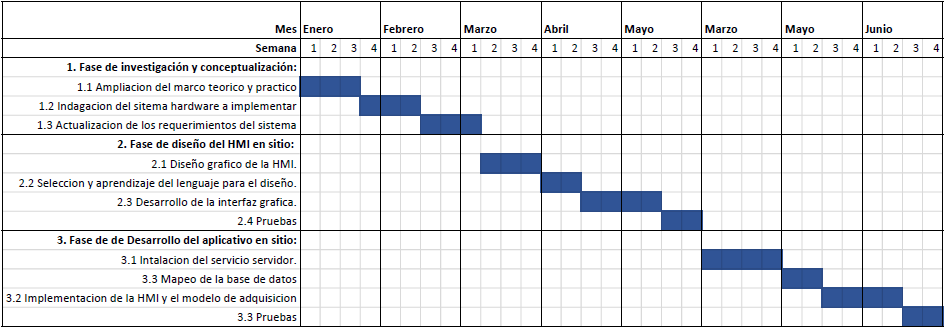
\includegraphics[width=15cm]{figuras/cronograma1.PNG}
	\caption{Cronograma de actividades periodo Enero - Junio}	
	\label{Cronograma periodo Enero - Junio}
\end{figure}

\begin{figure}[htbp]
	\centering
		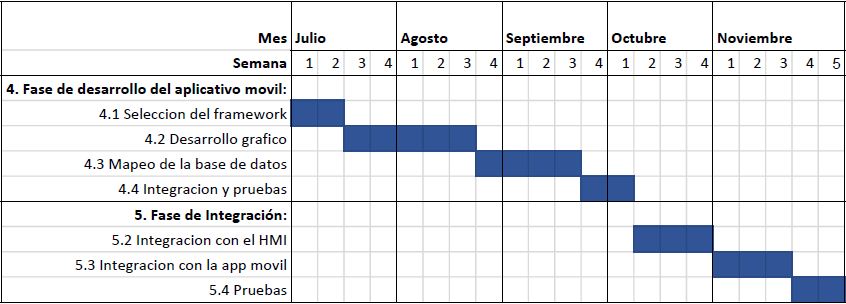
\includegraphics[width=15cm]{figuras/cronograma2.PNG}
	\caption{Cronograma de actividades, periodo Julio - Noviembre}	
	\label{Cronograma periodo Julio - Noviembre}
\end{figure}
%\section{Presupuesto}

\begin{figure}[htbp]
	\centering
		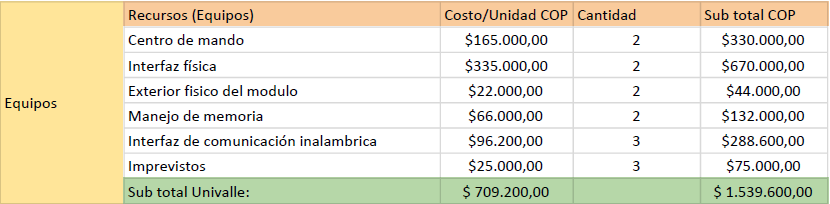
\includegraphics[width=15cm]{figuras/presupuesto_fisico.PNG}
	\caption{Presupuesto, materiales}	
	\label{Presupuesto, materiales }
\end{figure}

\begin{figure}[htbp]
	\centering
		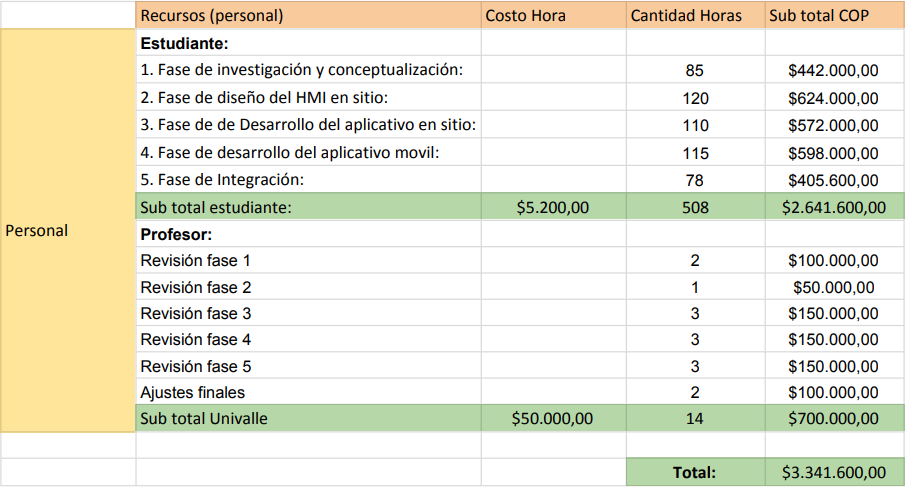
\includegraphics[width=15cm]{figuras/presupuesto_mano_de_obra.PNG}
	\caption{Presupuesto, mano de obra}	
	\label{Presupuesto, mano de obra}
\end{figure}



\customsection{Api de animación}
\subsection{Investigación y conceptualización}
Después de imaginar y delimitar  y el problema a tratar, cómo primera instancia, se seleccionó el tipo de entorno de trabajo que sería utilizado para el desarrollo del aplicativo ejecutable de manera local en la vivienda del Solar Decathlon. Durante el transcurso del documento este programa será llamado ``House Manager''.
\vspace{0.5cm}\\
Para seleccionar el entorno de trabajo se realizó una averiguación de los posibles entornos de desarrollo que permitieran implementar programación orientada a objetos en dispositivos embebidos, dentro de los entornos de desarrollo más conocidos se observó: Python, Java, Procesing, C++, entre otros. Todos los anteriores con comunidades muy enfocadas a su mejoramiento constante. Teniendo en cuenta lo anterior realizo un análisis por separado como se puede observar a continuación:
\begin{itemize}
	\item En el caso de C++ se observó que el entorno de trabajo más apropiado para desarrollar aplicativos gráficos era .net, la desventaja de este aplicativo era su estrecha relación con el lenguaje de programación de bajo nivel c\#, por ende el manejo de memoria del programa incrementa en gran medida los costos de desarrollo.
	\item Para Python se observó que los entornos de desarrollo de interfaz gráfica nativos tenían apariencias precarias similar a la nativa de Windows 98, en adición, los frameworks más estéticos tenían un soporte independiente al del lenguaje de programación como tal, por otra parte el lenguaje de programación como tal era multiplataforma y de muy alto nivel, lo que le permitiría al programador desarrollar algoritmos de mayor funcionalidad con menos líneas de código.
	\item En el caso de Java se observó que el entorno de desarrollo para interfaces gráficas era nativo del lenguaje de programación y permitía una mayor flexibilidad a la hora de desarrollar esquemas complejos con la excepción que se debía codificar detalladamente el comportamiento del objeto, lo que significaba más tiempo de trabajo para el programador y archivos con más líneas de código.
\end{itemize}
Como etapa de conceptualización, se realizó una primera versión el diseño del aplicativo principal junto con sus respectivas escenas (Fig \ref{fig_0}). Los elementos utilizados en esta primera etapa de diseño se consistieron principalmente de: botones, caja de opciones, contenedores, y paneles animados. Para esta etapa de conceptualización no se tenía una paleta de colores escogida pero si se buscaba tener en cuenta tonalidades verdes siendo congruentes con la temática amigable con el medio ambiente que rodea al Solar Decathlon, también, se persiguió el poder seleccionar a partir de la pantalla principal diferentes ``sub aplicativos'' que podrían ser diseñados de manera independiente.

\begin{figure}[htbp]
	\centerline{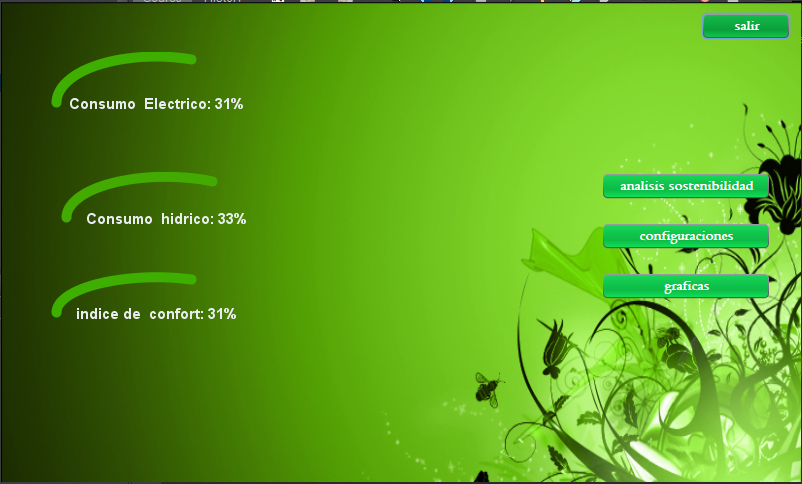
\includegraphics[width=8.5cm]{figuras/houseManager1.png}}
	\caption{Conceptualización inicial del api en sitio. Fuente: propia}
	\label{fig_0}
\end{figure}

Para hacer realidad el diseño de esta primera etapa de conceptualización se utilizó como lenguaje de programación el lenguaje de programación Java puesto que representaba en su mayor parte el lenguaje más utilizado en la Universidad del Valle durante el momento.

\begin{figure}[htbp]
	\centerline{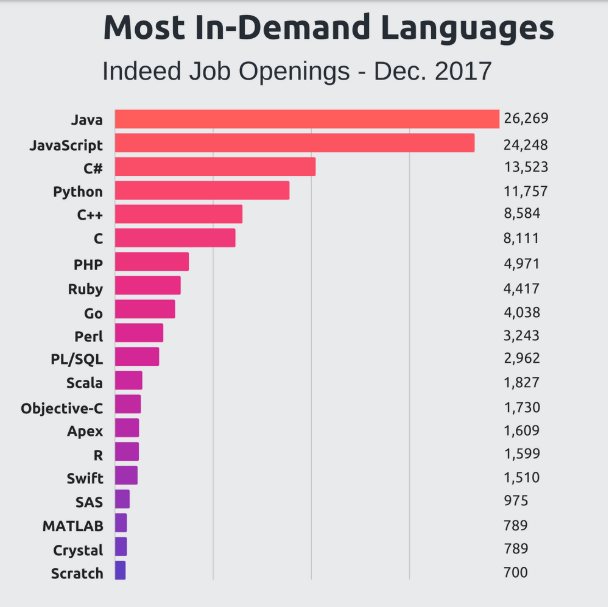
\includegraphics[width=8.5cm]{./figuras/stadistics_job.png}}
	\caption{Estadisticas de los lenguajes de programación con más demanda. Fuente: \cite{stackoverflow2017}}
	\label{fig_1}
\end{figure}

En adición, Java es un lenguaje de programación de muy alta demanda, de hecho, el de mayor ofertas de trabajo registradas durante el 2017 en el portal de trabajo internacional \href{https://co.indeed.com/?r=us}{indeed.com}, seguido de JavaScript, c\# y Python, tal como se observa en la figura \ref{fig_1}. Pero esta característica se debe principalmente a que el sistema bancario tradicional esta construido sobre servicios de backend utilizando Java.

\subsection{Api de java}
Todos los objetos implementados para la api fueron desarrollados estrictamente con java puro y sin librerías externas con el objetivo de obtener un código limpio, totalmente multiplataforma y que heredara paquetes únicamente de los módulos swing nativos de java. Como primera instancia se desarrolló el componente funcional de la API, es decir la parte programática, y finalmente se escribió el Javadoc, el cual es un documento integrado que describe como se deben usar los objetos 
\vspace{0.5cm}\\
Normalmente para java es necesario construir y empaquetar el código que contenga la interacción de manera manual con java puro. Por ejemplo, en JavaScript es posible enlazar funciones directamente sin acceder a paquetes adicionales como los ``event listeners'' de java, puesto que todo es considerado un objeto; desde un numero hasta una función.	
\vspace{0.5cm}\\
El primer objeto desarrollado en la api de java fue el botón personalizado, usando este objeto contenido en la api se puede crear un botón de cualquier tamaño con una, dos o tres imágenes para los estados; ``normal'', ``presionado'' y ``encima''. Un ejemplo de la utilización de la api se puede ver en la figura \ref{fig_2}. Este objeto funciona ajustando automáticamente su tamaño basado en la resolución de las imágenes, esto para complementar con una metodología de diseño: primero el dibujo, luego el programa.

\begin{figure}[htbp]
	\centerline{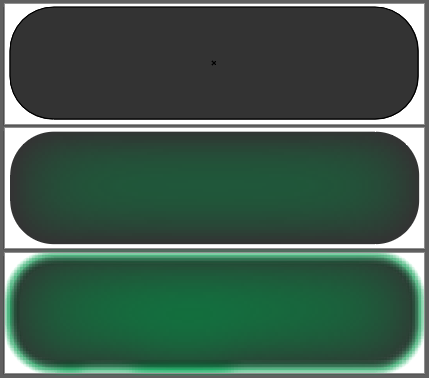
\includegraphics[width=8.5cm]{./figuras/boton.png}}
	\caption{El diseño de estados del botón interactivo. Fuente: propia}
	\label{fig_2}
\end{figure}

El segundo objeto grafico desarrollado fue un botón expandible o ``caja de opciones'', que permitiera generar un botón desplegable con la posibilidad de modificar texto de manera superficial basado en dos o tres imágenes para la parte superior, inferior y media respectivamente. Un implementación utilizada en la aplicación se puede observar en la figura \ref{fig_3}. Cada una de las imágenes del botón desplegable debe tener sus 3 imágenes de estado: normal, presionado y encima para interactuar de manera dinámica con el mouse.

\begin{figure}[htbp]
	\centerline{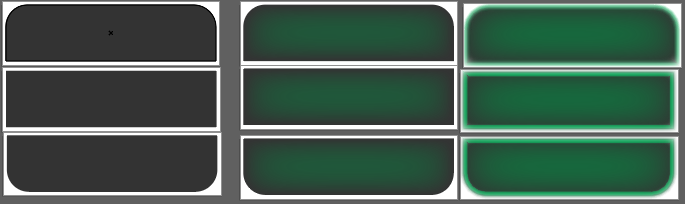
\includegraphics[width=7.5cm]{./figuras/boton_desplegable.png}}
	\caption{El diseño de los estados del botón interactivo desplegable. Fuente: propia}
	\label{fig_3}
\end{figure}

Como tercer objeto gráfico, se desarrolló un objeto de animación que podía mover un objeto tipo swing (esta es la clase madre de la mayoría de los objetos gráficos en java) en 4 posibles direcciones; las dos horizontales y las dos verticales, tal como se observa en la figura \ref{fig_4}. La función permite modificar la ubicación actual del objeto moviéndolo de manera linear con una rata de refresco dada (actualización visual) y una velocidad constante, desde una coordenada X o Y dependiendo de en cual eje coordenado se desee mover el componente.

\begin{figure}[htbp]
	\centerline{
\includegraphics[width=7.5cm]{./figuras/boton_movimiento.png}}
	\caption{Movimiento según la ubicación de la función horizontal. Fuente: propia}
	\label{fig_4}
\end{figure}

El desarrollo de la api fue de importancia para la construcción de la primera versión del aplicativo en sitio, la primera versión se puede observar en la figura \ref{fig_5}, debido a la recursiva implementación grafica se obtuvo un programa que sobrecargaba un sistema de cómputo completo (portátil Dell con procesador i5 segunda generación, 4gb de ram DDR3, y un disco duro HDD). Por lo tanto se buscó cambiar el entorno de desarrollo a uno con más flexibilidad a la hora del diseño gráfico, con capacidad de funcionar en sistemas de más bajo cómputo tipo Single Computer Boards como la Raspberry o la Beaglebone. Para probar el desempeño de la api, se realizaron pruebas con los elementos ya diseñados en la api de Java y se observó que resultaba una carga para el cpu realizar las animaciones, principalmente, cuando se deseaba mover más de 5 objetos tipo JavaSwing (los objetos gráficos nativos de java).

\begin{figure}[htbp]
	\centerline{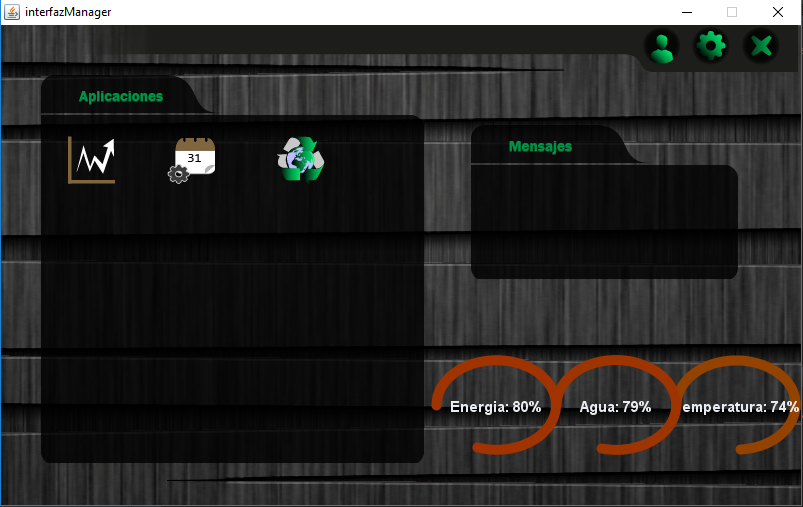
\includegraphics[width=8.5cm]{./figuras/houseManager23.png}}
	\caption{Primer Aproximación del diseño de la interfaz en sitio. Fuente: propia}
	\label{fig_5}
\end{figure}

Después de haber programado los elementos necesarios para generar la estructura básica del aplicativo se replanteo el diseño con una estructura más moderna y parecidas a las tendencias en diseño móvil tal como se observa en la figura \ref{fig_21} con el objetivo de que se percibiera que ambos aplicativos desarrollados en este sistema podían ofrecer los mismos servicios. Además, generar una experiencia de usuario similar en ambas plataformas

\begin{figure}[htbp]
	\centerline{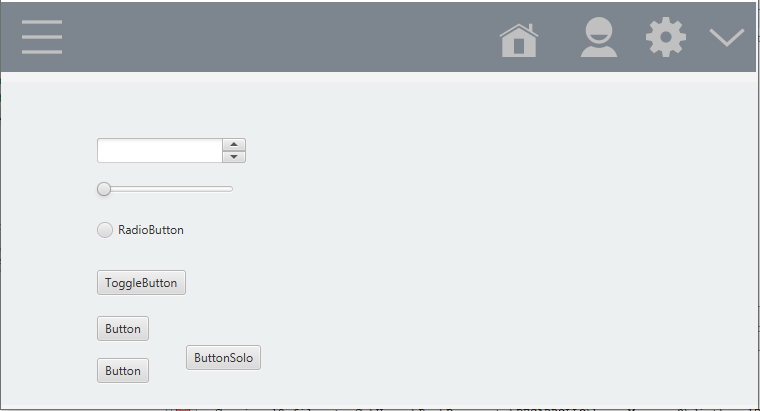
\includegraphics[width=8.5cm]{./figuras/house_manager_version_2.png}}
	\caption{Ajuste de diseño de la interfaz en sitio. Fuente: propia}
	\label{fig_21}
\end{figure}

En un tercer nivel de conceptualización se re diseño la interfaz gráfica estandarizando y simplificando los componentes que esta contenía; se seleccionó la paleta de colores y agregaron algunos nuevos objetos al diseño generalizado como se puede observar en la figura véase en la figura \ref{fig_22}. Para la correcta selección de la paleta de colores se buscó generar una simetría triangular en el espacio de colores HSV, usando como referencia un color sacado del logo oficial de la ``Chameleon House'' (nombre oficial de la casa diseñada para el Solar Decathlon). 

\begin{figure}[htbp]
	\centerline{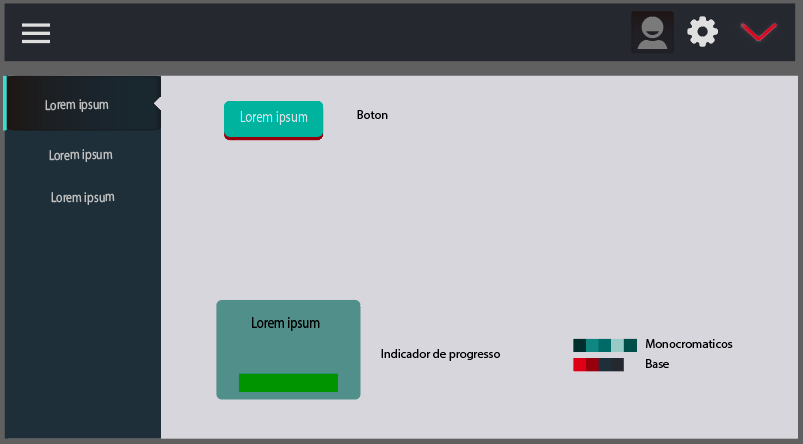
\includegraphics[width=8.5cm]{./figuras/house_manager_version_3.png}}
	\caption{Versión final del concepto de diseño. Fuente: propia}
	\label{fig_22}
\end{figure}

Debido a la estructura de Java, codificar todos los nuevos objetos resultaba una tarea de mayor trabajo y con baja recompensa, es decir, más líneas de código por objeto; como solución se tradujo lo que se tenía desarrollado hasta el momento de la api a un lenguaje de programación de más alto nivel (Python) y se utilizó un framework exclusivamente para el desarrollo de la interfaz gráfica, debido a que se trataba de un módulo completamente escrito en C le permitía a la aplicación tener un mejor rendimiento gráfico, con la desventaja de dificultar el efecto multiplataforma de Python, para mantener el efecto, el framework debería soportar por completo la plataforma sobre la cual se estuviera corriendo (Windows, macos, Linux, Ubuntu, etc).

\subsection{Api de Python y Qt}

El framework utilizado para desarrollar los módulos gráficos se llama Qt y para poder utilizarlo es necesario instalar unas dependencias C específicas y la librería respectiva para Python. Una vez Qt está correctamente configurado el diseño estatico del aplicativo se realiza a partir de un ``lenguaje de marcado'' (markup language) autogenerado llamado Qml que define las propiedades graficas estáticas de los objetos a utilizar, el Qml viene de la mano con un lenguaje tipo ``hoja de estilo'' (style sheet) llamado Qss, a partir del cual se le adjudican propiedades interactivas y estilos que en conjunto son comprendidos por Python y su librería Pyside. El anterior entorno de desarrollo, facilito la impllementacion de la api puesto que se relacioinaba directamente con la forma como se desarrolla frntend para la web.
Para esta etapa de diseño se utilizó una paleta de colores complementarios para los objetos importantes y tonalidades oscuras de grises azulados para los fondos. Todos dentro del espectro de colores de la marca de la casa del Solar Decathlon Latinoamerica de la Universidad del Valle.

Teniendo en cuenta el nuevo framework se utilizó la herramienta de diseño de Qt desing (oficial del framework) para codificar de manera automática las propiedades estáticas de la interfaz gráfica. También, se codificaron manualmente las propiedades dinámicas en un archivo de Qss que luego fue cargado por la librería Pyside para ser procesado como un objeto Python. 
\vspace{0.5cm}\\
Primero, se codificó un botón de la misma manera como se implemento el código de la API para Java; con este objeto de Python se logro crear un botón de cualquier tamaño con una, dos o tres imágenes para los estados; ``normal'', ``presionado'' y ``encima''. Un ejemplo de la utilización de la api se puede ver en la figura \ref{fig_19}.
\vspace{0.5cm}\\
\begin{figure}[htbp]
	\centerline{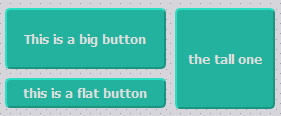
\includegraphics[width=7.5cm]{./figuras/qt_button.png}}
	\caption{Botón de tamaño flexible genérico de la api de qt. Fuente: propia}
	\label{fig_19}
\end{figure}

Segundo se codificó un botón genérico con las mismas funcionalidades del botón anterior, pero en lugar de funcionar basado en imágenes funcionaba con un color dado y las interacciones ``normal'', ``presionado'' y ``encima'' son calculadas atenuando y resaltando el color para generar un efecto de sombra e iluminación. Para el aplicativo se utilizó el color mostrado en la figura \ref{fig_20}.
\vspace{0.5cm}\\
Tercero, se desarrolló un expandible o ``caja de opciones'', personalizada, para ello se modificó el objeto de Qss “QOptionbar” que permite generar un botón desplegable con la posibilidad de modificar texto de manera superficial basado en un color especifico.
\vspace{0.5cm}\\
Cuarto, se programó una barra deslizable para facilitar el proceso de ingresar datos numéricos a la aplicación desde una interfaz táctil. Nuevamente se usaron los colores de la paleta de colores seleccionada y se optó por la solución de diseño más sencilla posible tal como se puede ver en la imagen \ref{fig_20}.

\begin{figure}[htbp]
	\centerline{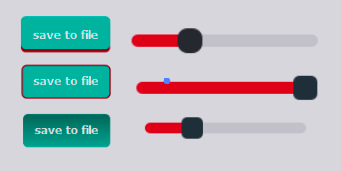
\includegraphics[width=7.5cm]{./figuras/qt_button_slide.png}}
	\caption{Boton de tamaño fijo usando imagenes y slider. Fuente: propia}
	\label{fig_20}
\end{figure}

Finalmente se personalizaron los colores de todos los espacios y elementos secundarios utilizados, como: la gráfica, la barra de menú, los botones especiales del menú, etc.



\customsection{House Manager}

Una vez descritos todos los componentes gráficos necesarios para realizar la aplicación, se implementaron los objetos de modelo, vista y controlador, basándose en los requerimientos descritos en la hoja ``requerimientos funcionales'' de la tabla \ref{tab0}. Para el desarrollo de estos componentes fueron necesarias diferentes condiciones técnicas que serán descritas en el siguiente apartado.

\subsection{Especificaciones técnicas}

La aplicación fue desarrollada utilizando el paradigma MVC, para ello, se organizo el proyecto en 3 carpetas: \textit{view, control y model}, donde todos los componentes y \textit{scripts} son gestionados desde un archivo principal. Debido a la naturaleza gráfica del proyecto y las limitaciones técnicas del hardware raspberry, se utilizó Python 2.7 para garantizar la compatibilidad de la mayor cantidad de sistemas operativos y librerías. 
Para el desarrollo de la aplicación fueron utilizadas las siguientes librerías:

\begin{itemize}
	\item \textbf{Paho-mqtt:} Esta librería se utilizó para establecer la comunicación con el bróker de Mqtt nativo de “Google Cloud Iot”.
	\item \textbf{Numpy, Scipy:} Estas listrerias fueron utilizadas para facilitar el procesamiento de vectores y mejorar el tiempo de procesamiento de los mismos.
	\item \textbf{Pyqtgraph:} Fue utilizada para gestionar el renderizado de las gráficas con el mejor valor posible de fotogramas por segundo. La necesidad de optimizar el componente grafico fue de importancia puesto que se desarrollaría sobre una tarjeta de computación de propósito específico (Raspberry).
	\item: \textbf{Http.client:} Esta librería fue utilizada para establecer una comunicación basada en solicitudes http con un ``endpoint'' del backend.
	\item: \textbf{Pyjwt, Cryptography:} Con esta librería se desarrolló la etapa de encriptación de datos adicional basada en \textit{Java Web Tokens}.	
\end{itemize}


Pensando en la escalabilidad del sistema, se definió un espacio para las ``aplicaciones'' adicionales donde se pudieran incluir nuevas rutinas de adquisición y control para dispositivos nuevos \ref{fig_6}. Como prueba de concepto se utilizó una rutina serial para adquirir el valor de khw acumulado en un contador eléctrico bifásico Inelca. Respecto a esta consideración de diseño se hablará más en el capitulo de ``pruebas y resultados''.
\vspace{0.5cm}\\

\begin{figure}[htbp]
	\centerline{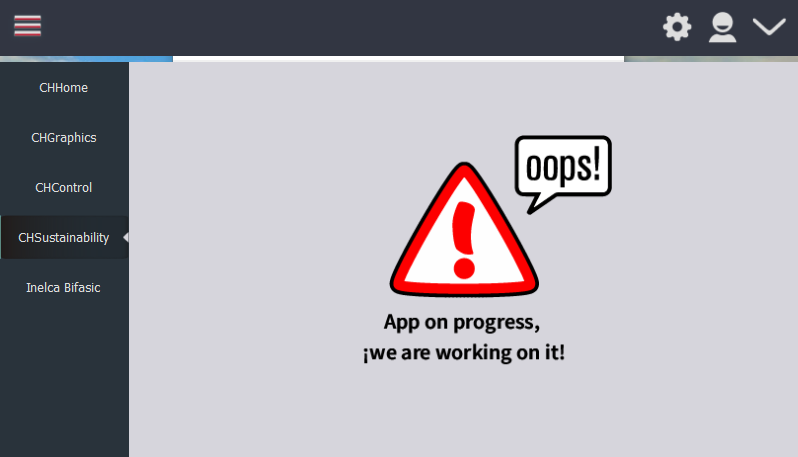
\includegraphics[width=8.5cm]{figuras/housemanager_newapp.png}}
	\caption{Visualización de la escalabilidad del sistema con una App no desarrollada por completo. Fuente: propia}
	\label{fig_6}
\end{figure}

En adición, se diagramó la experiencia de usuario de tal forma que el control y la medición de los dispositivos conectados a la tarjeta tuvieran el mismo ``costo de interacción'', es decir, que ambos estuvieran a la misma cantidad de clicks desde cualquier ventana del sistema. Por ende, todas las aplicaciones adicionadas en versiones futuras serán más fáciles de asimilar para el usuario.

\subsection{Requerimientos Funcionales}

Durante la etapa de conceptualización del proyecto de ingeniería que precede este documento se establecieron unos requerimientos funcionales con el fin de guiar el proceso de desarrollo. Este documento se puede ver el la tabla \ref{tab0}, y la implementación de cada requerimiento se puede observar a continuación:

\begin{figure}[htbp]
	\centerline{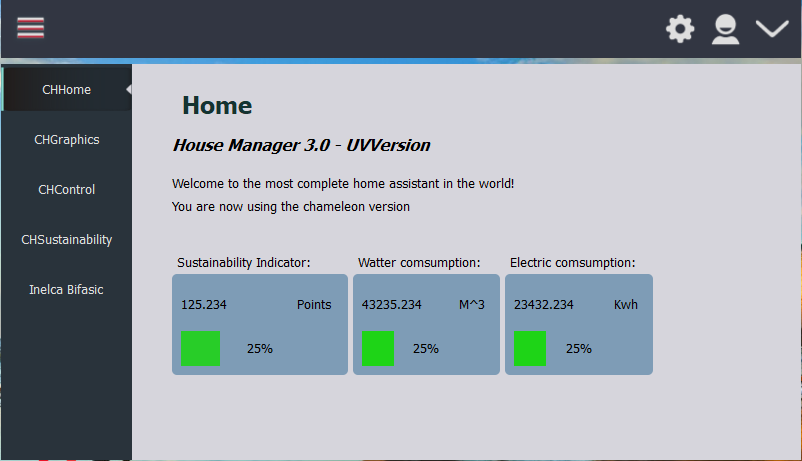
\includegraphics[width=8.5cm]{figuras/housemanager_home.png}}
	\caption{Escena del home del House Manager con barras de progreso para la indicación dinámica. Fuente: propia}
	\label{fig_7}
\end{figure}

\begin{enumerate}
	\item \textsl{``El sistema debe mostrar gráficamente la cantidad de agua y potencia consumida durante el día contrastándolas con un valor máximo recomendado'':} Para el desarrollo de esta funcionalidad se utilizó un componente gráfico tipo barra de progreso donde su 100 por ciento tenía como referencia la cantidad de agua recomendada para el número de personas presentes en la vivienda\ref{fig_7}. El número de personas presentes en la vivienda fue un dato ingresado manualmente por configuración inicial (sobre el sistema de configuración se hablará en los siguientes apartados de este capítulo).
	
	\item \textsl{``Por defecto el uso de las cargas eléctricas más significativas debe programarse durante los picos de generación en la casa, estos horarios podrán ser modificados bajo una advertencia de uso no eficiente'':} En miras de implementar esta funcionalidad se utilizó un elemento gráfico tipo calendario para configurar de manera individual las ventanas de activación de las cargas eléctricas en la vivienda\ref{fig_8}.
	\vspace{0.5cm}\\ 
	También, se consideró la opción de activación o desactivación inmediata de los circuitos; para ello se, implementó una rutina flexible que permitió ignorar las cargas eléctricas que el usuario había modificado manualmente (Esta rutina se nombró ``Scheduler Handler''), lo anterior únicamente durante 24 horas para no afectar el objetivo de sostenibilidad de la vivienda. 
	\vspace{0.5cm}\\
	Además, se utilizó la conexión Mqtt para accionar remotamente cualquiera de los circuitos localmente gestionados, en caso de recibir un mensaje de control para los circuitos el sistema también suspendiera por 24 horas la acción del ``Schedule Handler''.
	\item: \textsl{``El usuario debe poder acceder a la información medida en tiempo real'':} Para la implementación de este requerimiento se creo una ventana gráfica con la capacidad de mostrar el valor de la medida del sensor con un tiempo de muestreo entre 1 y 50 Hertz. Teniendo en cuenta lo anterior, el medidor debe ser capaz de almacenar el valor de consumo eléctrico y de agua internamente. Tal como lo hace el contador eléctrico bifasico de Inelca con el que se realizaron las pruebas.
	\vspace{0.5cm}\\
	Si el usuario lo desea, puede cambiar el numero de puntos y la frecuencia de muestreo de manera inmediata, moviendo las barras deslizables. Ademas, puede guardar los datos mostrados en la gráfica en el formato de excel presionando el boton ``save to file''.
	\item: \textsl{``El sistema debe poder comunicarse con una base de datos que represente todas las variables y el estado de los circuitos de la vivienda'':} Para la implementación de este requerimiento se creo un ``endpoint'' en el servicio de \textit{backend} con la capacidad de hacer consultas de históricos a la base de datos (Un ``endpoint'' es un url web gestionado por un backend en el cual se pueden realizar solicitudes Http). La solución tiene este comportamiento puesto que la aplicación del cliente final no debe tener ningún tipo de credencial para el acceso a la información directamente, con una capa de procesamiento se pueden integrar este tipo de solicitudes con el mismo sistema de encriptacion del broker de Mqtts (para más información de los endpoints y la rutina de encriptacion vease el capitulo \textit{backend}).
\end{enumerate}


\begin{figure}[htbp]
	\centerline{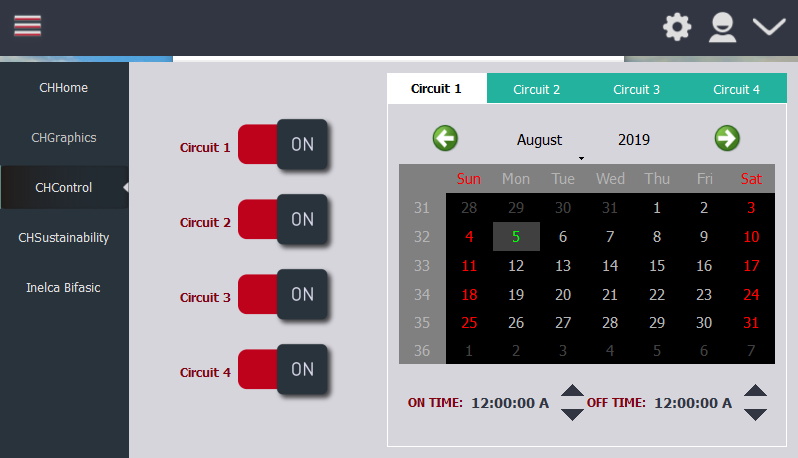
\includegraphics[width=8.5cm]{figuras/housemanager_control.png}}
	\caption{Escena de control del House Managern con sus calendarios. Fuente: propia}
	\label{fig_8}
\end{figure}

\subsection{Funciones adicionales}

En adición a los requerimientos funcionales, se añadieron funciones a la conceptualización de diseño original para mejorar el funcionamiento de la plataforma y la experiencia de usuario. Dentro de estas funciones podemos encontrar la configuración del sistema, la posibilidad de guardar localmente para no perder la información adquirida, etc. Para comprender mejor estas funciones adicionales, serán descritas a continuación:

\begin{enumerate}
	\item \textbf{Handler remoto:} Esta característica le permite al sistema cambiar de manera automática entre el modo remoto y el modo local para no perder información en ningún momento del reporte de datos. En caso de la caída repentina de la red, el programa es capaz de cambiar al modo local sin la perdida de ningún dato. También, es capaz de entender cuando el usuario desea que el dispositivo funcione permanentemente de manera local o cuando el sistema vuelve a estar nuevamente conectado a la red. Los datos que son guardados de manera local se almacenan en la carpeta personal del usuario, en archivos de excel, y son creados por dia con la fecha como nombre. Teniendo en cuenta lo anterior, el nivel de autonomia local depende exclusivamente de la memoria en el disco duro; para la Raspberry fueron aproximadamente 10 GB de las 16 disponibles en la memoria micro SD.
	
	\item \textbf{Sistema de almacenamiento local:} Con esta característica el House Manager puede almacenar todos los datos adquiridos en una hoja de Excel generando archivos organizados por días. También es capaz de almacenar en un archivo diferente los datos presentes en la gráficas teniendo en cuenta el día de adquisición. \ref{fig_9}.
	\begin{figure}[htbp]
		\centerline{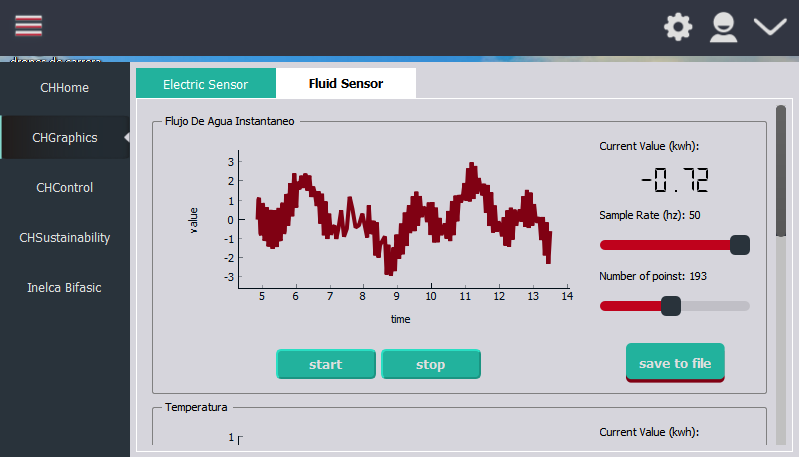
\includegraphics[width=8.5cm]{figuras/housemanager_measure.png}}
		\caption{Escena de medición del House Manager, con su respectivo panel para guardar los datos. Fuente: propia}
		\label{fig_9}
	\end{figure}

	\item \textbf{Ajustes de configuración} Esta es una característica que incluye una ventana adicional donde se configuran los aspectos concernientes al sistema en general\ref{fig_10}. Los aspectos configurables del sistema son: La frecuencia en segundos con la que se reportan los datos al servidor, el costo del kilo watt hora, el costo del metro cubico de agua, el día de notificación del correo (ver función ``Notificación automática''), el modo de funcionamiento (remoto o local) y el nombre de la ubicación (este nombre es opcional y sirve para administrar los diferentes dispositivos desde la perspectiva del backend).
	\begin{figure}[htbp]
		\centerline{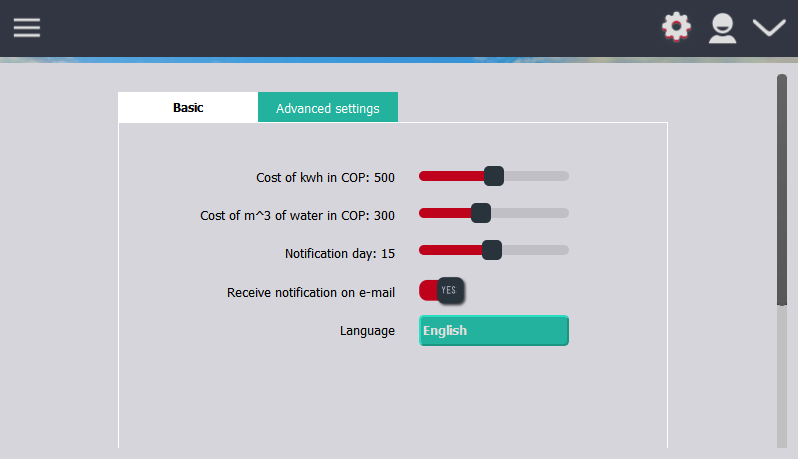
\includegraphics[width=8.5cm]{figuras/housemanager_config.png}}
		\caption{Escena de configuración del dispositivo House Manager. Fuente: propia}
		\label{fig_10}
	\end{figure}

	\item \textbf{Notificación Automática:} Para el correcto desarrollo de esta función se compró el dominio \href{www.alfagenos.com}{www.alfagenos.com} para recibir las notificaciones desde el remitente de correo: notificaciones@alfagenos.com. Esta notificación tendrá lugar dependiendo de la configuración establecida e indicara el gasto en pesos del consumo eléctrico y de agua hasta la fecha establecida en la configuración. También notificará los gastos  energéticos en horarios adicionales al pre establecido por la configuración del Solar Decathlon.
	
	\item\textbf{Autenticación usando google:} Para desarrollar esta funcionalidad se utilizó la api de autenticación de google y se creo una escena aparte para la visualización del usuario \ref{fig_11}.
	\begin{figure}[htbp]
		\centerline{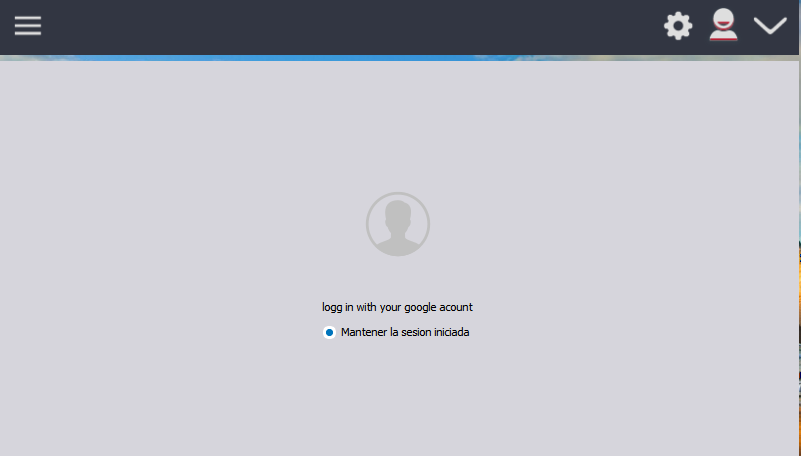
\includegraphics[width=8.5cm]{figuras/housemanager_user.png}}
		\caption{Escena para el inicio de sesión del House Manager. Fuente: propia}
		\label{fig_11}
	\end{figure}
	
	\item \textbf{Doble nivel de encriptación:} Debido a las exigencias de los servidores de Google se implementaron 2 capas de seguridad de encriptación para la  comunicación de la aplicación con el backend. La primera capa es de tipo Tls y opera para cualquier producto de google, inclusive las operaciones realizadas por los navegadores. La segunda se desarrolló usando encriptación ``RS256'' a través de Jwt.
\end{enumerate}

\subsection{Algoritmos Utilizados}

Para cumplir con algunos requerimientos funcionales y algunas funciones adicionales, fue implementar hilos de proceso en segundo plano que se encargaron de tareas que no eran sensibles a pequeños cambios en la frecuenciade ejecucion. Los algoritmos utilizados en estos hilos de programa, comparten la información de toda la aplicación a través de los 3 objetos principales: el controlador la vista y el modelo. Estos algoritmos o programas ocurren en segundo plano y no representan una carga significativa para el CPU ni se comportan de manera determinista respecto a los tiempos de ejecución establecidos para los mismos. 

\subsubsection{Scheduler Handler}
Este Hilo es el encargado de verificar y mantener el estado de los circuitos según ha sido configurado en la ventana del horario de manera automatica. Este hilo de programa es capaz de discernir los circuitos que se han activado de manera manual desde la aplicación móvil o desde la interfaz de escritorio. Ante un evento de estos (manual), la influencia de la ventana de activacion o desactivacion automatica se desactiva por 24 horas y el circuito entra en un modo manual por 24 horas.
.
\subsubsection{Remote Mode Handler}
Este hilo de programa está encargado de verificar el estado de la conexión con el servidor para cambiar el modo de almacenamiento de la información, si es necesario. Si el dispositivo se desconecta, el sistema de almacenamiento cambia a la memoria local y si vuelve la conexión el handler es capaz de conectarse automáticamente al broker web para reportar los datos nuevamente, sin perdida de información.

\subsubsection{Mail Notification Handler}

Este hilo es el encargado de verificar la fecha y realizar las notificaciones correspondientes al consumo eléctrico, el consumo de agua y el indicador de sostenibilidad. También, lleva el registro del consumo generado por fuera de los horarios recomendados por el Solar Decathlon.

\subsubsection{Data Report Handler}

Esta rutina es la encargada de reportar automáticamente los valores medidos y almacenados en las gráficas, esta rutina almacena datos con una periodicidad que va desde  cada segundo hasta cada 5 minutos. Como aclaración, cada vez que se reportan los datos de las gráficas, no se toman en cuenta todos los datos intermedios, por ende hay una perdida para variables de medición con una granularidad mayor a 1 segundo. En la figura \ref{fig_34} se puede observar que el periodo ``T1'' corresponde al tiempo de muestreo de alta granularidad a partir de la cual se grafican los datos en tiempo real en la ventana de medición; por otro lado, el periodo ``T2'' corresponde al tiempo de muestreo a partir del cual se guardan los datos en el servidor o en memoria.
\begin{figure}[htbp]
	\centerline{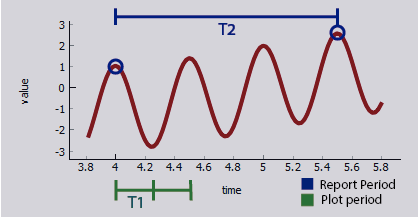
\includegraphics[width=8.5cm]{figuras/graph_explanation.png}}
	\caption{Descripción de los tiempos de muestreo utilizados en el sistema de adquisición. Fuente: propia}
	\label{fig_34}
\end{figure}

\subsubsection{Indicator Handler}

Esta es la rutina que se encarga de monitorear el estado de consumo eléctrico y de agua para modificar los valores de los indicadores de la ventana de inicio. Así como también, calcular el valor del indicador de sostenibilidad utilizando exclusivamente en el consumo eléctrico y de agua.


 

\customsection{Serverless backend}

Durante el desarrollo del \textit{backend} se evaluó la posibilidad de utilizar las alternativas de nube más reconocidas y con mayor facturación en el mercado actual; Lo anterior con el objetivo de implementar el desarrollo con el proveedor más confiable. Dentro de los posibles proveedores se evaluaron las siguientes opciones: Amazon Web Services, Google Cloud y Microsoft Azure. Los anteriores proveedores fueron escogidos por el tamaño que tienen en la industria; una mirada de la reparticion del mercado actual se puede observar en la figura \ref{label}


\begin{figure}[htbp]
	\centerline{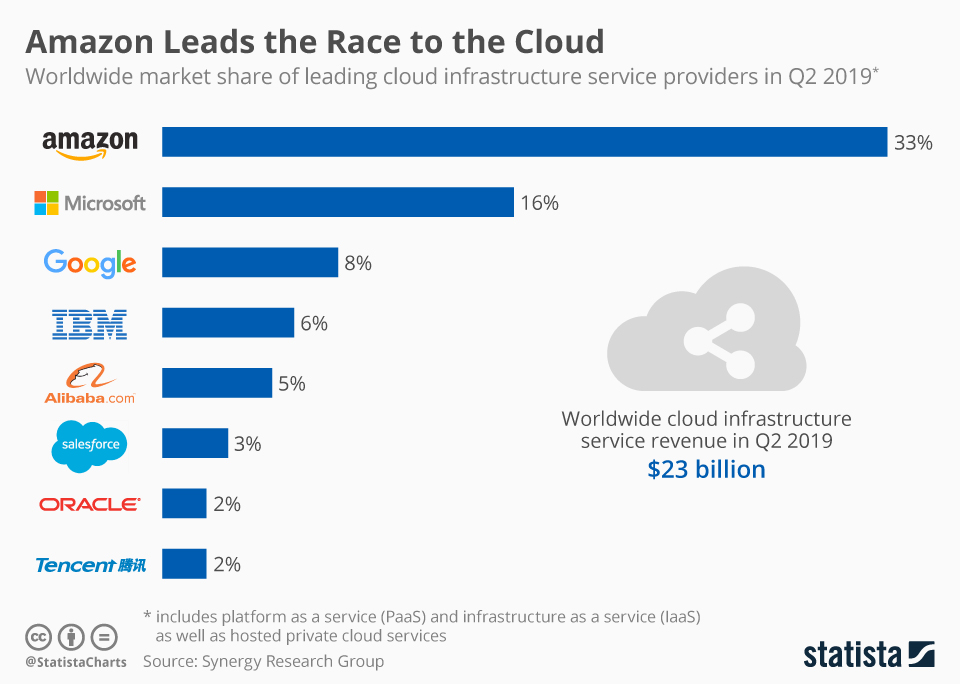
\includegraphics[width=12cm]{./figuras/market_share.jpg}}
	\caption{Estadística de la repartición del mercado de servicios de nube en 2019. Fuente: \cite{cloudstadistics}}
	\label{maket_stadistics}
\end{figure}

Teniendo en cuenta los tres proveedores mencionados anteriormente se pudo observar que los factores diferenciadores de cada uno, dependian estrictamente de los productos adicionales que estos ofrecían:
\vspace{0.5cm}\\
Por una parte, los servicios de nube de Amazon Web Services representan la mayoría del mercado de la nube, pero esto se debe en su mayoría al almacenamiento de información, por ende, tiene una gran variedad de servicios de nube, incluyendo sus tiendas en linea y sus servicios de storage webs. En resumen, Amazon posee la mayor variedad de servicios de nube en la actualidad.
\vspace{0.5cm}\\
Por otra parte, los servicios de Google incluyen el uso de su red privada que tiene el mejor desempeño en velocidad dentro del mercado. En adición, los servicios de Google Cloud poseen interfaces de administración con más experiencia de usuario y la posibilidad de integrar servicios de machine learning, big data y de procesamiento de audio.
\vspace{0.5cm}\\
Finalmente, Microsoft Azure es el servicio de nube con la posibilidad de integrarse de manera optima con los servicios como  Windows Server, Office, .Net, entre otros. Por otra parte la documentacion entorno a los servicios de microsoft Azure no es tan completas como las de los dos competidores anteriormente mencionados.
\vspace{0.5cm}\\
Cabe aclarar que al escoger a cualquiera de estos proveedores no resulta comprometido el uso de los servicios de otros: para integrar servicios de otro proveedor, solo se requiere establecer las condiciones apropiadas para autenticar nodos de red diferentes a los de las redes internas que los proveedores ya administran.
\vspace{0.5cm}\\
Teniendo en cuenta todo lo anterior, se escogió el servicio de nube de Google porque tiene los servicios de machine learning y de procesamiento de voz más avanzados. Por ende, aunque no se utilizan para esta version del proyecto, la integracion en futuros trabajos será más fluida. Además, debido a que el sistema operativo utilizado para probar la aplicacion celular es Android, la integracion de Google Cloud  y la ``User App'' será mas fácil.
\vspace{0.5cm}\\
Una vez escogida la plataforma de nube y el servicio de comunicación se decidió desarrollar el \textit{backend} tipo serverless para aprovechar todas las ventajas del servicio escalable de mensajes de internet de las cosas de Google llamado ``Cloud Iot''.

\subsection{Especificaciones técnicas}

Para el montaje del modelo de la nube se utilizaron principalmente 4 componentes: la base de datos MySql, el servicio de almacenamiento por contenedores tipo ``Storage 3'' de Amazon, el servicio de Cloud IOT como bróker de internet de las cosas y las ``Cloud Functions'' del servicio de servidores de Google. De los elementos anteriormente mencionados se puede entender el backend como una serie de funciones que son activadas con eventos tipo solicitudes Https y mensajes basados en Mqtts, por ende todo el flujo de información será orquestado por las funciones que se definan en el sistema. El flujo de la información se puede observar más adelante en la sección ``funciones de nube''. Adicionalmente, Un diagrama generalizado de los componentes del \textit{backend}, se puede ver en el capitulo de diseño en la figura \ref{diagramaGeneralizado}. 
\vspace{0.5cm}\\
Las funciones de nube de Google operan como scripts de lenguajes de programación como Node.js, Python y Golang; estas requieren de librerías para operar de manera efectiva con cualquier componente del sistema. Para el desarrollo de este modelo se decidió utilizar el entorno de desarrollo de Node.js, puesto que era un lenguaje de programación familiar y de alto nivel. Teniendo en cuenta lo anterior, para poder hacer uso de los componentes necesarios para implementar el sistema diseñado se utilizaron las siguientes librerías:

\begin{itemize}
	
	\item \textbf{``@Google-cloud/storage'':} Esta librería es desarrollada y mantenida por google y permite hacer uso de las descargas, las subidas y la administración de los servicios de almacenamiento de archivos ``Cloud Storage''.
	
	\item \textbf{``Mysql'':} La librería oficial de MySql para Node.js, con esta librería se implementó la comunicación con la base de datos MySql y se crearon todas las rutinas para guardar y obtener datos en la base de datos.
	
	\item \textbf{``Googleapis'':} Esta librería es la encargada de comunicarse directamente con cualquier dispositivo conectado a la red, fue utilizada para reenviar los mensajes recibidos por los dispositivos a través del puente ``Cloud Iot''.
	
	\item  \textbf{``Jsonwebtoken''} Esta librería fue utilizada para autenticar los mensajes recibidos por las solicitudes Https y Mqtts, a partir de las llaves públicas de los dispositivos registrados en el sistema. El algoritmo de encriptación utilizado fue el RSA256.
	
	\item  \textbf{``Google-auth-lib''} La librería de autenticación de google fue utilizada para obtener las credenciales necesarias para utilizar el puente de Iot del proyecto.
	
\end{itemize}


\subsection{Base de datos relacional y no relacional}

Una parte muy importante del \textit{backend} es la base de datos y, aunque el sistema de almacenamiento de ``Cloud Storage'' funciona como un disco duro con todas las facilidades para majear archivos naturales, tiene limitaciones y costos asociados al número de operaciones de lectura y escritura que se pueden hacer en el mes. Por el contrario, la base de datos MySql tiene costos asociados únicamente con el tamaño del almacenamiento y la capacidad del procesador; debido a esto es la opción más apropiada para almacenar datos de pequeño tamaño pero de gran cantidad.
\vspace{0.5cm}\\
El diseño de la base de datos estuvo apoyado por el programa de administración de bases de datos: \textsl{``MySql Workbench''}. Un esquema generalizado de la base de datos se puede observar en el diagrama \ref{fig_23}, donde cada cuadro representa un grupo de tablas bajo el paradigma SQL. 
\vspace{0.5cm}\\

\begin{figure}[htbp]
	\centerline{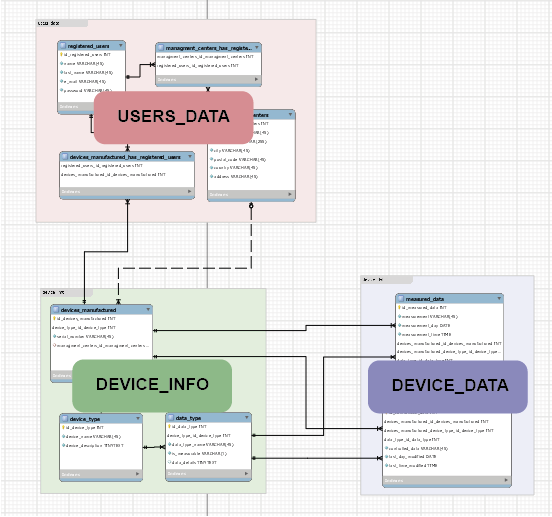
\includegraphics[width=15cm]{figuras/UML.png}}
	\caption{Diagrama general de la base de datos relacional MySql. Fuente: propia}
	\label{fig_23}
\end{figure}

Teniendo en cuenta lo anterior, se explicará por separado cada grupo de tablas con el objetivo de mostrar las escalabilidad del sistema y como fue implementada la base de datos pensando en los requerimientos funcionales de los productos House Manger y User App. cabe aclarar que para representar los tipos de campos se utilizaron los siguientes símbolos: un bombillo amarillo significa que se trata de una columna de llave primaria única, un rombo azul representa un buffer de tipo \textit{char} obligatorio, un rombo blanco significa buffer de tipo \textit{char} no obligatorio y los campos sin símbolo son llaves secundarias de relación obligatorias.


\begin{itemize}
	
	\item \textbf{Users data:} Figura \ref{fig_25}. En este grupo de tablas se encuentran principalmente 2 tablas:
	\vspace{0.5cm}\\
	La tabla registered\_users, que almacena la información de los clientes; esta información consta de un correo de registro y un espacio para la ``contraseña''. Realmente el espacio de la contraseña es una entrada para una ``llave privada'' generada por Google que se utiliza para acceder a la información personal de los usuarios desde el \textit{backend}.
	\vspace{0.5cm}\\
	La tabla managment\_centers, que agrupa los dispositivos fabricados en regiones de operación; en esta tabla se tiene como objetivo referenciar a los usuarios y los dispositivos a una zona horaria GTM y una descripción de dirección. Esta tabla presenta una utilidad representativa en el caso de realizar envíos o referenciar espacios geográficos en los cuales se encuentran los dispositivos.
	\vspace{0.5cm}\\
	Finalmente, Las tablas adicionales son las tablas de relación muchos a muchos de un paradigma SQL relacional.
	
	\begin{figure}[htbp]
		\centerline{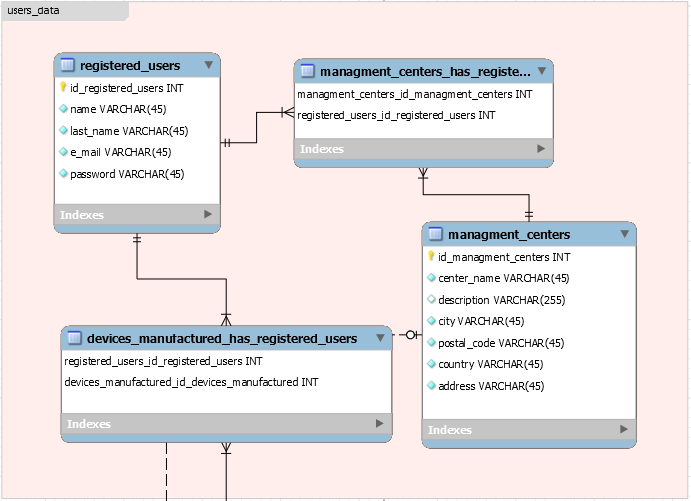
\includegraphics[width=7cm]{figuras/users_data.png}}
		\caption{Grupo de tablas: users data. Fuente: propia}
		\label{fig_25}
	\end{figure}
	
	\item \textbf{Device\_info:} Figura \ref{fig_26}. En este grupo existen 3 tablas y todas contienen información relevante: La tabla devices\_manufatured contiene principalmente el número serial de un dispositivo para identificarlo a los ojos del fabricante. La tabla device\_type contiene una breve descripción del dispositivo y su nombre. Por último, la tabla  data\_type sirve para almacenar la información de todas las posibles variables medibles y los actuadores configurables para todos los dispositivos, este ultimo campo es para garantizar que el sistema pueda explicarse por si mismo con una simple consulta. Teniendo en cuenta que el sistema puede recibir dispositivos que no han sido fabricados de manera propia, juntando el nombre y el numero serial, se obtiene una identificación única por sensor o actuador conectado al sistema. 
	
	\begin{figure}[htbp]
		\centerline{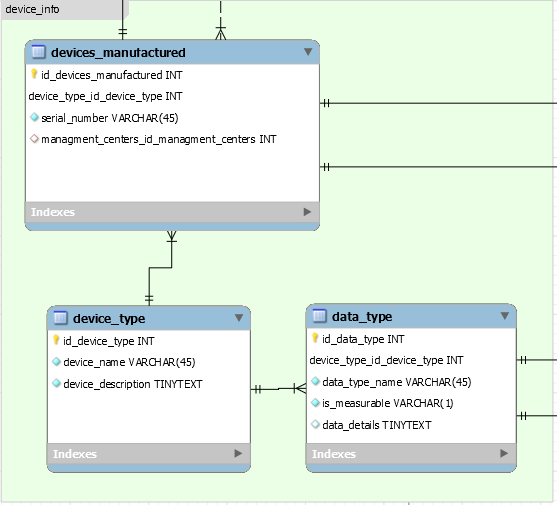
\includegraphics[width=7cm]{figuras/device_info.png}}
		\caption{Grupo de tablas: device info}
		\label{fig_26}
	\end{figure}
	
	\item \textbf{Device\_data:} Figura \ref{fig_27}. El grupo de tablas de información se compone únicamente de 2; la tabla measured\_data contiene la información que fue medida y tiene una estampa de tiempo de mínimo 1 segundo, la tabla controllable\_data contiene las estampas de tiempo en las cuales se le dio la orden al dispositivo modificar su actuador de forma específica. Teniendo en cuenta lo anterior, un valor de control en un momento especifico no garantiza que ese actuador se haya modificado de esa forma en el centro de gestión; garantiza que el dispositivo estaba conectado a la red y recibió el comando de hacerlo.
	
	\begin{figure}[htbp]
		\centerline{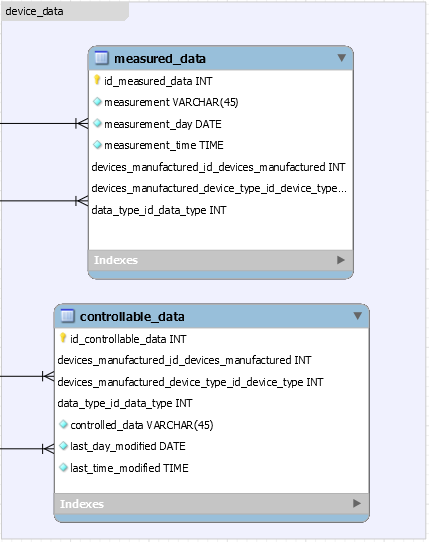
\includegraphics[width=7cm]{figuras/device_data.png}}
		\caption{Grupo de tablas: device data. Fuente: propia}
		\label{fig_27}
	\end{figure}
	
\end{itemize}

Finalmente el componente no relacional del sistema de almacenamiento tipo ``Storage 3'' funciona como un sistema de archivos y tiene como interfaz la api propia de google anteriormente mostrada. Internamente para almacenar la información de los usuarios se organizó la información en carpetas con el nombre ``sql\_uid{id mysql}'' donde el texto ``{id mysql}'' corresponde a la llave primaria única entera utilizada para identificar a los usuarios en la base de datos relacional (la columna llamada ``id\_registered\_users'' de la tabla ``registered\_users'')
\vspace{0.5cm}\\
Teniendo en cuenta la estructura de almacenamiento anteriormente mencionada, el sistema obtiene su cuello de botella en el número de conexiones MySql que puede recibir, todos los demás elementos pueden escalar, en teoría, de manera infinita. Para la versión de la base de datos que se está utilizando se pueden permitir 4000 conexiones simultaneas, por ende, se dice que el sistema está diseñado para 4000 dispositivos.

\subsection{Relación de requerimientos funcionales}

Debido a que este producto no se contempló en la estaba de conceptualización y planeación del proyecto no tuvo una lista de requerimientos funcionales sobre los cuales crear scripts o funciones, por el contrario, los requerimientos funcionales de los otros dos productos: El House Manager y el User Manager exigían un desarrollo desde la perspectiva del \textit{backend}. Teniendo en cuenta lo anterior, se explicaran los desarrollos realizados en el \textit{backend} y los requerimientos funcionales que pretendían solucionar.

\begin{enumerate}
	\item \textsl{``El usuario debe poder acceder a la información medida en tiempo real''.} Para cumplir este objetivo fue necesario crear un puente de conexión en tiempo real de un dispositivo a otro, siendo el segundo un dispositivo de monitoreo como lo es la User App. El puente es realizado por el “cloud iot” y a travez de una función de nube que es activada cada vez que se reporta un valor de medición (esta función será explicada más adelante)
	\item \textsl{``El usuario debe poder acceder al histórico del mes y la relación de sus gastos con ellos''.} Como solución a este requerimiento se diseñó una REST API (aquel conjunto de funciones basadas en solicitudes Http, que se utilizan para ofrecer un servicio en específico) capaz de obtener datos de la base de datos de medición o control entre un periodo de tiempo específico. 
\end{enumerate}


\subsection{Funciones de nube}
Una función de nube es una rutina de código que se ejecuta cada vez que se realiza una solicitud Https o se recibe un mensaje directamente desde Google (como es en el caso del broker de IOT; ver figura \ref{diagramaGeneralizado} para ver bloques funcionales del \textit{backend}) y esta función puede retornar un mensaje en formato de texto si asi lo desea.
Teniendo en cuenta lo anterior, las funciones de nube implementadas en este sistema tienen como características: una memoria ram de 512 megabytes, la posibilidad de tener acceso a una memoria volátil temporal únicamente existente durante el tiempo de ejecución de la función y la posibilidad de ejecutar los lenguajes de programación: Node.js, Python y Go. Cabe aclarar que este tipo de arquitectura posee como limitación un límite de ejecución por función de 9 minutos. Las anteriores características fueron configuradas directamente en la plataforma de Google y se encuentran dentro de los valores gratuitos del servicio.
\vspace{0.5cm}\\
Teniendo en cuenta lo anterior, se implementaron 4 funciones de nube que le permitieron al sistema cumplir con los requerimientos funcionales. Estos cada una de las funciones serán explicadas en los siguientes apartados.

\subsubsection{Get\_historical\_data:}

Esta función fue diseñada para recibir un mensaje a través de un ``post request''. El contenido del post debe ser buffer codificado a 64 bits con un objeto de JavaScript (Json) convertido. El contenido de este objeto debía ser el necesario para: validar la legitimidad de la solicitud, conocer el tipo de dato que se desea obtener de la base de datos, el dispositivo del cual se desea conocer la información y el rango de tiempo en el que se desean consultar los datos. Teniendo en cuenta lo anterior un ejemplo del objeto Json aceptado como argumento de la función es:
\begin{Verbatim}[tabsize=4]
{
	"type":"control",
	"sql_uid":1,
	"number_points": 10,
	"device_name": "House Manager SDL"
	"serial_number": 1000023211
	"data_type": "potencia activa instantanea",
	"init_date": "2019-07-18",
	"final_date": "2019-08-12",
	"encripted_token": "SsidfmjEFShfDBGSsdEFSBzdfw3RQEfassdg23"
}
\end{Verbatim}
Donde  el campo ``type'' es opcional y tiene como valor por defecto los datos de medición, el campo ``sql\_uid'' corresponde al identificador único de usuario de la base de datos, el campo ``number\_points'' corresponde al número máximo de puntos que puede tener el objeto de respuesta, ``serial\_number'' es el numero serial del dispositivo que genero los datos que se desean obtener, ``data\_type'' es un string con el nombre del tipo de dato registrado en la tabla data\_type, los campos ``init\_date'' y ``final\_date'' representan los límites temporales en los cuales se debe realizar la consulta.
\vspace{0.5cm}\\
Por último, el campo ``encripted\_token'' se debe incluir un Sting encriptado conteniendo el objeto de autenticación. El Sting debe estar encriptado utilizando el algoritmo de Rivest–Shamir–Adleman de 256 bits y el objeto descifrado debe contener la siguiente información:

\begin{Verbatim}[tabsize=4]
{
	iat: 1234232009,
	exp: 1236323009
}
\end{Verbatim}


Donde ``iat'' es un entero con el número de milisegundos en los cuales se creó el token, teniendo en cuenta, un punto de referencia de la maquina (Enero 1 de 1970 a la hora 00:00:00 UTC.) y el campo ``exp'' es también un entero con los milisegundos en los cuales expira el token, de autenticación, teniendo en cuenta el mismo punto de referencia.
\vspace{0.5cm}\\
Debido a que el sistema de autenticación basado en los JWT es el mismo en todas las funciones no será explicado nuevamente en las siguientes secciones, solo serán explicados los campos nuevos o los que tengan un significado diferente.
\vspace{0.5cm}\\
El algoritmo de la función se puede separar en 5 pasos generales, fig \ref{fig_28}, cada uno de los pasos se puede ver a continuación:
\begin{figure}[htbp]
	\centerline{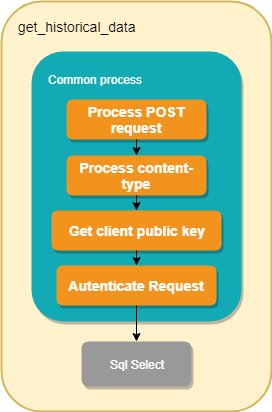
\includegraphics[width=6cm]{figuras/algoritmo_get_historical.png}}
	\caption{Algoritmo de la función: Get historical data. Fuente: propia}
	\label{fig_28}
\end{figure}
\begin{enumerate}
	\item \textbf{Segmentacion del tipo de request:} En esta etapa de la función se verifica que la solicitud sea unicamente de tipo POST
	\item \textbf{Segmentacion por formato de mensaje:} En esta etapa se verifica que el tipo de contenido del mensaje sea ``application/json''
	\item \textbf{Adquisicion de la llave publica:} Para autenticar el usuario se accede al servicio de almacenamiento S3 para optener la llave ``verificadora'' del usuario en cuestión.
	\item \textbf{Autenticación de usuario:} Se descifra el token de acceso y se verifica que el token no se encuentre vencido.
	\item \textbf{Consulta SQL:} Se utiliza la información contenida en el mensaje para realizar una consulta SQL dependiendo del tipo de operación y se organizan los datos en un objeto resultado.
\end{enumerate}
Teniendo en cuenta el proceso anterior, un ejemplo del objeto resultante de solicitud Http a esta función es:

\begin{Verbatim}[tabsize=4]
{
	``data\_type'': ``potencia activa instantanea,
	"data": [
		{
			"data": "1213123",
			"date": "2019-06-12",
			"time": "17:44:51",
		},
		{
			"data": "333123",
			"date": "2019-07-12",
			"time": "3:12:11",
		}
	]
}
\end{Verbatim}
Donde el objeto es un Json codificados en base 64 del objeto convertido a Sting. el contenido de "data" depende del número de puntos que se soliciten y el campo "data\_type". Teniendo en cuenta el vector de datos de ejemplo, cabe aclarar que toda la información temporal recibida esta referenciada a la zona horaria cero (UTC: 0).

\subsubsection{Send\_command:}

Esta función también fue diseñada para recibir un mensaje a través de un "post request". y también debe recibir un buffer codificado a 64 bits con un objeto de JavaScript (Json) convertido. La razón por la cual se escogió el "POST" como el tipo de solicitud fue puesto que con las solicitudes post el servidor en cuestión encripta la información usando su certificado de seguridad SSL, es decir, que en este caso la información transmitida esta encriptada con el certificado SSL de Google.
\vspace{0.5cm}\\
Teniendo en cuenta que la función también fue diseñada basada en un post y con todos los requerimientos de encriptación y codificación, un ejemplo de un mensaje seria:
\begin{Verbatim}[tabsize=4]
{
	"sql_uid": 1,
	"mqtt_sub_folder": "control/raspberry",
	"operation": "send-save",
	"encripted_token": "SsidfmjEFShfDBGSsdEFSBzdfw3RQEfassdg23",
	"message":{
		"some_json_object"
	}
}
\end{Verbatim}
Dado el anterior objeto Json: el campo de ``mqtt\_sub\_folder'' define el tema al cual el dispositivo  de recepción está suscrito. El campo ``operation'' contiene una de las siguientes opciones; send-save, send o save y controla la operación que debe realizar el \textit{backend} con el mensaje. En caso de ser save, solo guardará en la base de datos el mensaje enviado (este mensaje debe contener la información necesaria para guardarse en la base de datos; si no tiene el formato indicado, no será guardado en la base de datos a pesar de que si sea enviado y recibido por el dispositivo). En caso de solo ser send, el \textit{backend} le enviara un mensaje al dispositivo, si es posible, y finalizara la operación. Finalmente, si la operación es send-save el \textit{backend} intentará enviarle un mensaje al dispositivo, si lo recibe, asume que la variable de control fue modificada y guarda en mensaje en la base de datos.
\vspace{0.5cm}\\
El campo message contiene el mensaje que recibirá el dispositivo, teniendo en cuenta que el mensaje es para la modificación de una variable de control el mensaje debe contener la estampa de tiempo en la que se generó la orden, el valor al cual se desea modificar la variable y el tipo de data a la cual corresponde la información. Un ejemplo de Json con la capacidad para almacenar la información de la orden es:
\begin{Verbatim}[tabsize=4]
"some_json_object" = {
	"device_name": device_name,
	"serial_number": serial_number,
	"data_type": ["control circuito a", "control circuito b"],
	"data": ["off","on"],
	"date": ["2019-06-12", "2019-07-12"],
	"time": ["3:12:11", "3:12:40"],
}
\end{Verbatim}
Como se puede observar anteriormente, los campos de "data", "date" y "time" contienen un vector, lo que le permite a esta función realizar múltiples operaciones SQL y modificar múltiples actuadores con una sola solicitud.
\vspace{0.5cm}\\
El resultado de esta operación es un objeto tipo Json con la información de la operación SQL, es decir, información como el número de filas afectadas, el tiempo que tomo la operación, entre otros. Para más información de este objeto se puede revisar la documentación oficial de la librería de mysql \cite{mysql}.
\vspace{0.5cm}\\
Adicionalmente, un diagrama generalizado del algoritmo se puede ver en la figura \ref{fig_29}. Teniendo en cuenta esta figura el algoritmo de la función se puede dividir en 6 pasos:

\begin{figure}[htbp]
	\centerline{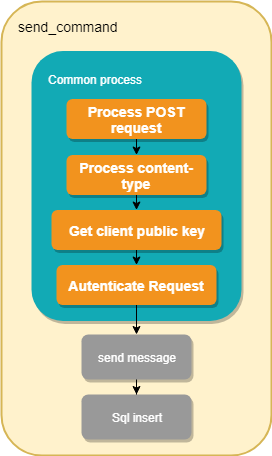
\includegraphics[width=6cm]{figuras/algoritmo_send_command.png}}
	\caption{Algoritmo de la función: Send command. Fuente: propia}
	\label{fig_29}
\end{figure}

\begin{enumerate}
	\item \textbf{Segmentación del tipo de request:} Al igual que en la función anterior se discrimina para que solo se acepten solicitudes tipo ``POST''
	\item \textbf{Segmentación por formato de mensaje:} Así como en la función ``get\_historical\_data, se rechazan las solicitudes que no tengan como formato de contenido ''application/json''.
	\item \textbf{Adquisicion de la llave publica:} También, hacemos la consulta al servicio de almacenamiento para adquirir la llave pública que será usada en el proceso e descifrado.
	\item \textbf{Autenticación de usuario:} Nuevamente Se descifra el token de acceso y se verifica que el token no se encuentre vencido.
	\item \textbf{Envío del mensaje Mqtt:} Se envía exactamente el contenido del campo mensaje al dispositivo de interés usando el tópico especificado en el campo (``mqtt\_topic'')
	\item \textbf{Registro de la información:} si el dispositivo está conectado y ha recibido correctamente el mensaje, se guarda la información del mensaje en la base de datos, si el mensaje no tiene el formato indicado este último paso no se realiza.
\end{enumerate}

\subsubsection{IOT\_gateway\_control:}

Esta función es muy diferente a las otras dos funciones explicadas anteriormente; por el contrario a ellas, esta función es activada o ejecutada a través de un sistema de publicación y suscripción interno de Google Cloud (``pub/sub message system'') para comunicar sus diferentes dependencias. En el momento que un bróker Mqtt recibe una publicación bajo el tema ``control'' un evento de pub/sub se genera, y por consiguiente, esta función de nube que está asociada a él. 
\vspace{0.5cm}\\
Adicionalmente, el proceso y funcionamiento de la función puede considerarse igual al de las otras dos funciones con pequeños cambios, todo el proceso de autenticación es manejado directamente por el servicio de ``Cloud Iot'', por ende el campo ``encripted\_token'' ya no se encuentra en los mensajes recibidos. Un ejemplo de un mensaje enviado por un dispositivo a través de una publicación Mqtt es:
\begin{Verbatim}[tabsize=4]
{
	"sql_uid": 1, 
	"mqtt_sub_folder": "control/raspberry",
	"operation":"send-save",
	"message":{
		"device_name": "House Manager SDL",
		"serial_number": 1000000000,
		"data_type": ["circuito 1","circuito 2"],
		"data": ["on", "off"],
		"date": ["2019-06-12", "2019-10-0"],
		"time": ["17:44:51", "21:00:51"],
	}
}
\end{Verbatim}
Teniendo en cuenta el Json anterior se puede observar que su formato es muy parecido al del objeto de la función ``send\_command'' con la diferencia que no contiene el campo de objeto encriptado, esto se debe a que el objeto encriptado es utilizado como contraseña al momento de establecer la conexión con el bróker desde el cliente. En adición, un diagrama generalizado del algoritmo se puede ver en la figura \ref{fig_30}. Teniendo en cuenta esta figura el algoritmo de la función se puede dividir en 4 pasos:

\begin{figure}[htbp]
	\centerline{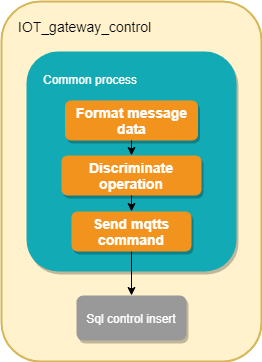
\includegraphics[width=6cm]{figuras/algoritmo_iot_control.png}}
	\caption{Algoritmo de la función: Iot gateway control. Fuente: propia}
	\label{fig_30}
\end{figure}
\begin{enumerate}
	\item \textbf{Organizar el mensaje:} Los mensajes recibidos por el broker Mqtt de Google tienen un formato tipo ``buffer'', por lo tanto, en esta etapa se convierte el arreglo recibido en un formato interpretable por el sistema.
	\item \textbf{Discriminación de operacion:} Asi como se discriminó en la funcion ``Send\_command'' en este campo se describe el tipo de operacion que se debe realizar con el mensaje. La operacion será ``send-save'' por defecto
	\item \textbf{Envío del mensaje de control Mqtt:} Se envia exactamente el contenido del campo mensaje al dispositivo de interés a travez de su tema (``mqtt topic'').
	\item \textbf{Registro de la información:} si el dispositivo está conectado y ha recibido correctamente el mensaje, se guarda la información del mensaje en la base de datos, si el mensaje no tiene el formato indicado este último paso no se realiza.
\end{enumerate}

\subsubsection{IOT\_gateway\_measure:}

Esta función comparte todos sus pasos con la anterior, es decir que es muy parecida desde una perspectiva general; la diferencia se encuentra en el último paso de la misma, un diagrama generalizado de este algoritmo se puede ver en la figura \ref{fig_31}. En el último paso, si todos los anteriores fueron completados exitosamente, el algoritmo intenta guardar la información en la tabla de control de la base de datos.

\begin{figure}[htbp]
	\centerline{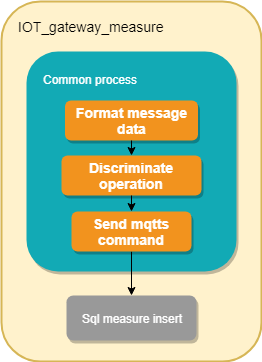
\includegraphics[width=5cm]{figuras/algoritmo_iot_measure.png}}
	\caption{Algoritmo de la función: Iot gateway measure. Fuente: propia}
	\label{fig_31}
\end{figure}

Adicionalmente, la función debe recibir un Json con el mismo formato que el recibido por ``iot\_gateway\_control'' con diferencias en sus campos: ``data\_type'' y ``mqtt\_sub\_folder'', puesto que en el tipo de dato debe contener el identificador de la variable de control y en mqtt\_sub\_folder debe haber un Sting que identifique el tópico Mqtt que el dispositivo destino pueda reconocer como un mensaje de control. 
\vspace{0.5cm}\\
Para efectos prácticos, en esta etapa de la implementación, con el objetivo de discernir un tipo de mensaje de otro se escogió como formato de tema: ``{nombre}/control'', donde {nombre} es el nombre del dispositivo al cual se le desea enviar el mensaje. Con esto, no se quiere decir que el tema Mqtt esté ligado a este formato, en el caso que se deseen escalar los comandos y añadir más actuadores a un dispositivo ya diseñado, se puede modificar el sistema de temáticas propuesto para esta versión de los productos \textit{backend}.


\customsection{User app}

Teniendo en miras de la escalabilidad deseada para este sistema se escogió el framework de desarrollo de aplicaciones móviles llamado React Native. Este es un framework de JavaScript desarrollado y mantenido por Facebook Inc con ventajas significativas desde la perspectiva de diseño: permite desarrollar aplicaciones nativas para Android y iOS a través de un sistema de traducción de componentes desde JavaScript al lenguaje nativo de la maquina (Java para Android y Swift para IOS), por ende, las aplicaciones desarrolladas en este framework tienen un desempeño muy similar a las implementadas directamente en los lenguajes nativos correspondientes.
\vspace{0.5cm}\\
En adición, una ventaja estratégica que tiene el desarrollar aplicaciones a través de este framework es que ambos desarrollos (para IOS y Android) quedan con las mismas interfaces gráficas, lo que le da al cliente la misma experiencia de usuario sin importar en que plataforma se encuentre.
\vspace{0.5cm}\\
Aunque desarrollar aplicaciones para Android y IOS con el mismo lenguaje de programación suena extremadamente ventajoso, hay limitaciones técnicas que serán mencionadas más adelante en este capítulo.

\subsection{Especificaciones técnicas}

Para poder realizar el aplicativo se utilizaron diferentes librerías de JavaScript creadas específicamente para el framework de React-Native. Las librerías utilizadas en el aplicativo fueron:

\begin{itemize}
	\item \textbf{React-native-google-signin:} Esta librería fue utilizada para obtener las llaves privadas y la información de usuario utilizando el servicio de autenticación de Google.
	\item \textbf{React-native-progress:} Con esta librería se lograron desarrollar los indicadores de progreso circulares para mostrar el índice de consumo eléctrico de agua y el coeficiente de sostenibilidad.
	\item \textbf{Jsrsasign:} Usando esta librería fue posible encriptar los JWT de autenticación a partir del protocolo de RSA de 256 bits. Esta librería fue de vital importancia puesto que poseía toda la compatibilidad necesaria para ser ejecutada con JavaScript puro, sin el uso de paquetes adicionales escritos en Java o Swift.
	\item \textbf{React-native-svg:} Esta librería fue utilizada para apoyar el desarrollo de componentes visuales adicionados a las gráficas.
	\item \textbf{React-native-svg-charts:} Usando esta librería fue posible integrar gráficas en el aplicativo móvil.
	\item \textbf{React-native-swiper:} Con esta librería se implementó la interfaz tipo deslizante (``swipe'') en las ventanas de introducción de la aplicación.
	\item \textbf{React-native-vector-icons:} Con esta librería fue posible utilizar los iconos nativos de Android y IOS como el botón de menú, de home, entre otros.
	\item \textbf{Toggle-switch-react-native:} Con esta librería se implementaron botones conmutadores (on off), utilizados en la escena de control.
	\item \textbf{React-navigation:} Esta librería fue utilizada para establecer el control de la navegación y el menú dentro de la aplicación como se puede ver en la figura \ref{fig_17}.
	\item \textbf{React-redux:} Usando esta librería fue posible comunicar de manera efectiva todos los objetos y componentes del sistema.
	\item \textbf{Fetch:} Con esta librería se estableció la comunicación basada en solicitudes Https con el backend.
\end{itemize}
\begin{figure}[htbp]
	\centerline{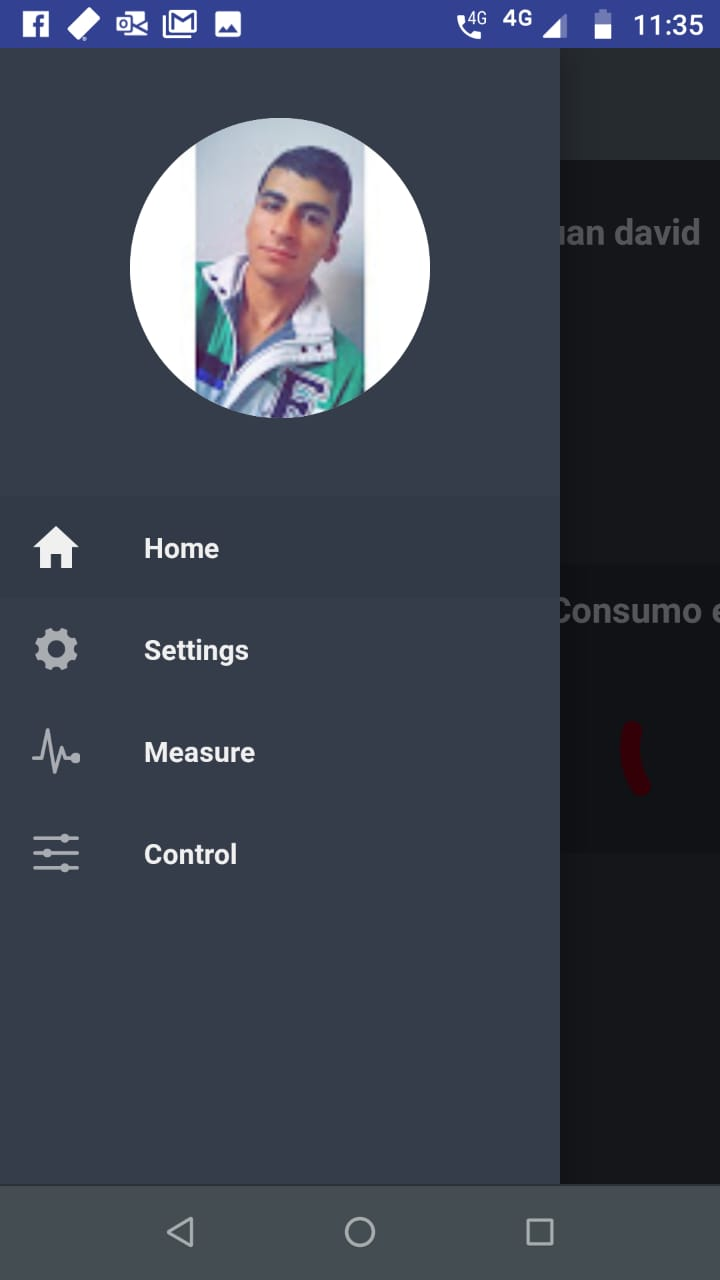
\includegraphics[width=6cm]{./figuras/mobile_menu.jpeg}}
	\caption{El menú desplegable con las aplicaciones actualmente desplegadas. Fuente: propia}
	\label{fig_17}
\end{figure}
Teniendo en cuenta que React\_native traduce todos sus componentes al lenguaje nativo del celular, es necesario entender que no todas las librerías de JavaScript se pueden usar para el framework, únicamente aquellas que tienen incluido el enlace de bajo nivel con ambos sistemas operativos. Por ende, las librerías con mayor compatibilidad son las que están desarrolladas exclusivamente con JavaScript puro. 
\vspace{0.5cm}\\
Con la anterior consideración en mente, en el proceso de desarrollo se presentó un problema por asumir incorrectamente que un ``snipet'' (Archivo o script que cumple una función en específico) era capaz de funcionar en el entorno de programación de React-Native. Este pequeño ``snipet'' fue desarrollado pensando en integrar las funcionalidades del protocolo de comunicación Mqtts a la aplicación; pero usaba librerías que estaban basadas en paquetes de bajo nivel equivocados, es decir, para computadores de uso comercial como linux o windows. Por ende, las funcionalidades de tiempo real fueron implementadas utilizando únicamente el protocolo de comunicación Https.
\vspace{0.5cm}\\
Para finalizar, de las librerías utilizadas, se puede observar que la mayoría son para mejorar la interfaz gráfica, mejorar la experiencia de usuario u obtener la misma vista entre sistemas operativos Android y Ios.

\subsection{Requerimientos Funcionales}

Debido a que durante el proceso de planeación del proyecto también se utilizó la herramienta de RUP para definir las especificaciones de esta aplicación, y estos requerimientos guiaron el proceso de desarrollo, se explicará cómo se implementaron las especificaciones establecidas:

\begin{enumerate}
	\item \textsl{``El usuario debe poder acceder a la información medida en tiempo real:''} Para solucionar este requerimiento, en una primera etapa de desarrollo, se optó por utilizar una librería llamada ``react-native-mqtt''. Esta librería funcionaria como puente entre las librerías: ``Paho Mqtt Client' de Android y ``Mqtt Framework'' de IOS, pero debido al estado tan pionero de las tecnologías de desarrollo de React Native y el protocolo de comunicación Mqtt, la librería no era estable y muchas otras similares tampoco. 
	\vspace{0.5cm}\\
	Teniendo en cuenta lo anterior se implementó la comunicación en ambos sentidos a través de las solicitudes Https, por ende, para obtener los datos en tiempo real en la aplicación le realiza solicitudes al backend de tal forma que reciba los últimos datos guardados en el sistema de almacenamiento MySql.
	\vspace{0.5cm}\\
	Finalmente, para mostrar la información medida en tiempo real se implementó la escena de medición ``measure'' tal como se ve en la figura \ref{fig_15}, donde deslizándose hacia abajo se puede tener acceso a las gráficas con contenido de otros sensores.
	\begin{figure}[htbp]
		\centerline{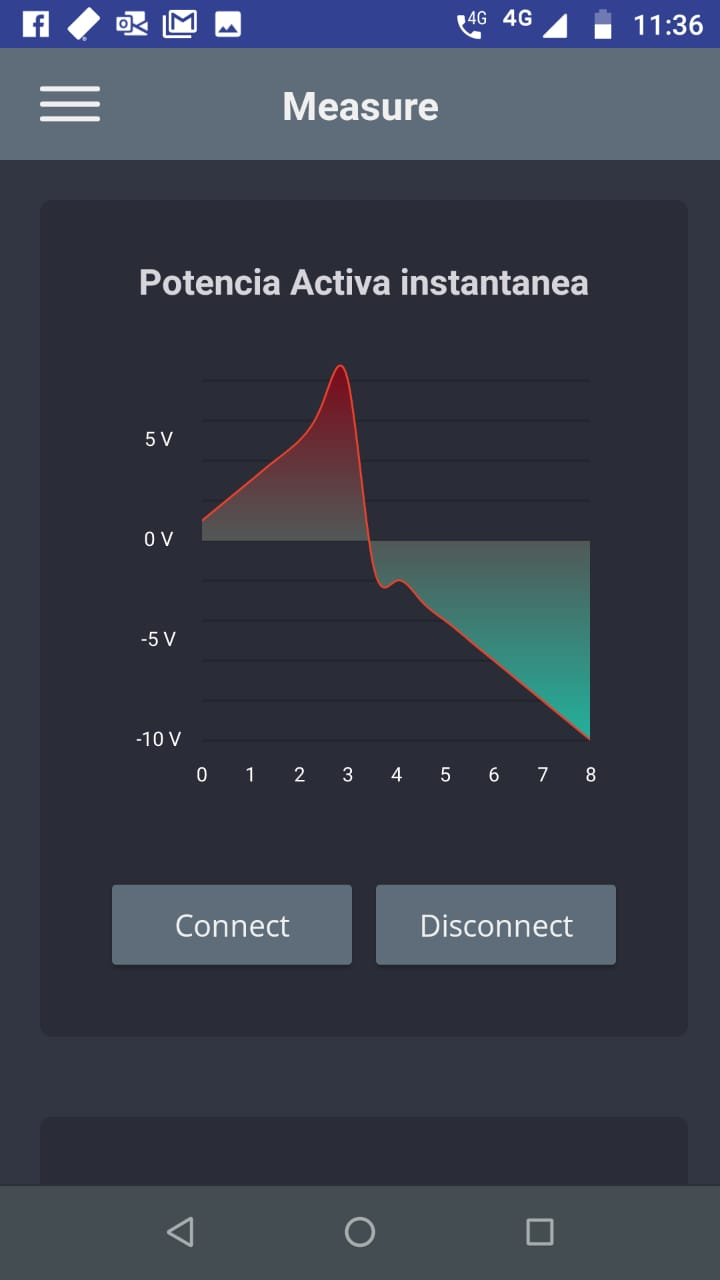
\includegraphics[width=6cm]{./figuras/mobile_measure.jpeg}}
		\caption{Escena para la medición en tiempo real de las variables. Fuente: propia}
		\label{fig_15}
	\end{figure}
	\item  \textit{``El usuario debe ser capaz de cambiar los parámetros de configuraciones establecidos por defecto para la vivienda del solar Decathlon:''} Por defecto los parámetros de la vivienda del Solar Decathlon involucran unos horarios de uso de las cargas eléctricas, por ende, cuando el usuario realiza un cambio en la aplicación celular el sistema en sitio desactiva su configuración predeterminado. 
	\vspace{0.5cm}\\
	Finalmente, se implementó una escena de configuración. Esta escena, no se añadió ninguna entrada de usuario y se dejó para ilustrar la posibilidad de incluirlo en el futuro. La escena se puede observar en la figura \ref{fig_18}.
	
	\begin{figure}[htbp]
		\centerline{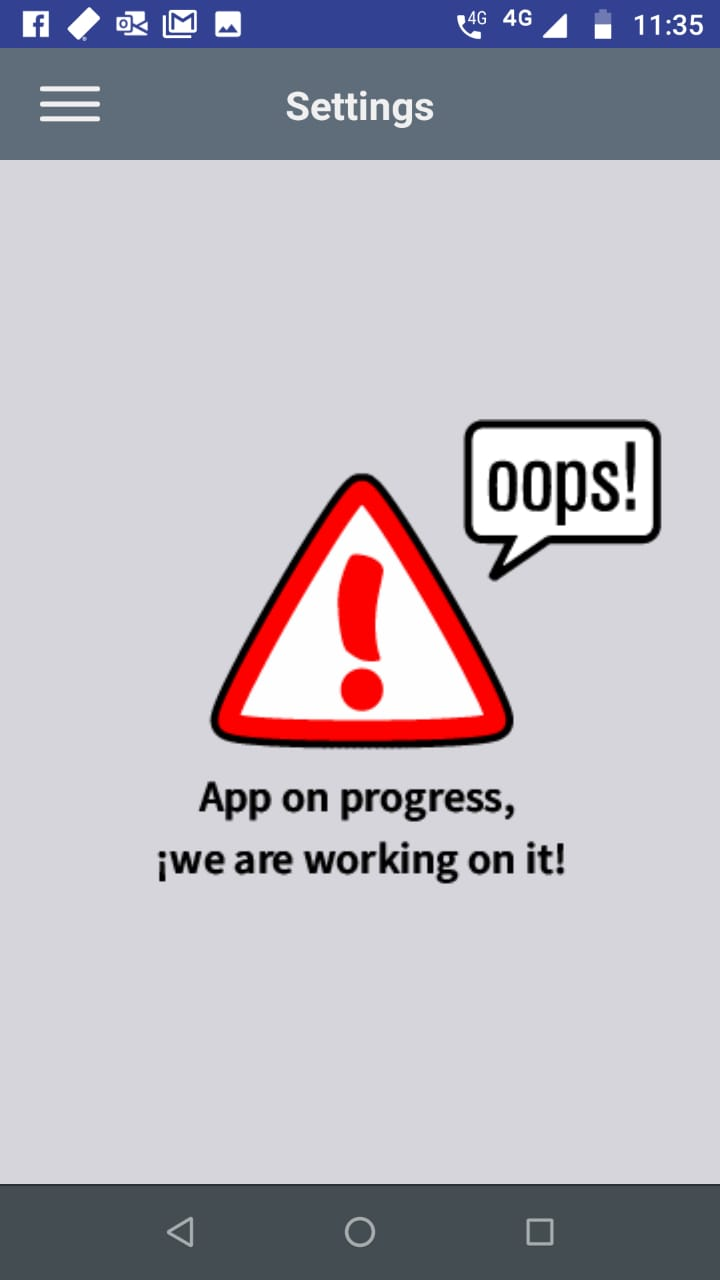
\includegraphics[width=5cm]{./figuras/mobile_settings.jpeg}}
		\caption{Escena de configuraciones, actualmente no disponible. Fuente: propia}
		\label{fig_18}
	\end{figure}
	
	\item \textit{``El usuario debe poder acceder al histórico del mes y la relación de sus gastos con ellos:''} Para implementar este requerimiento se utilizaron barras circulares de progreso que indican la cantidad de energia o agua que ha consumido el usuario en el día, comparándola con un valor promedio. La escena desarrollada para solucionar este requerimiento se puede ver en la figura \ref{fig_13} donde el usuario puede panear horizontalmente el centro de la pantalla para revelar los otros indicadores.
	\begin{figure}[htbp]
		\centerline{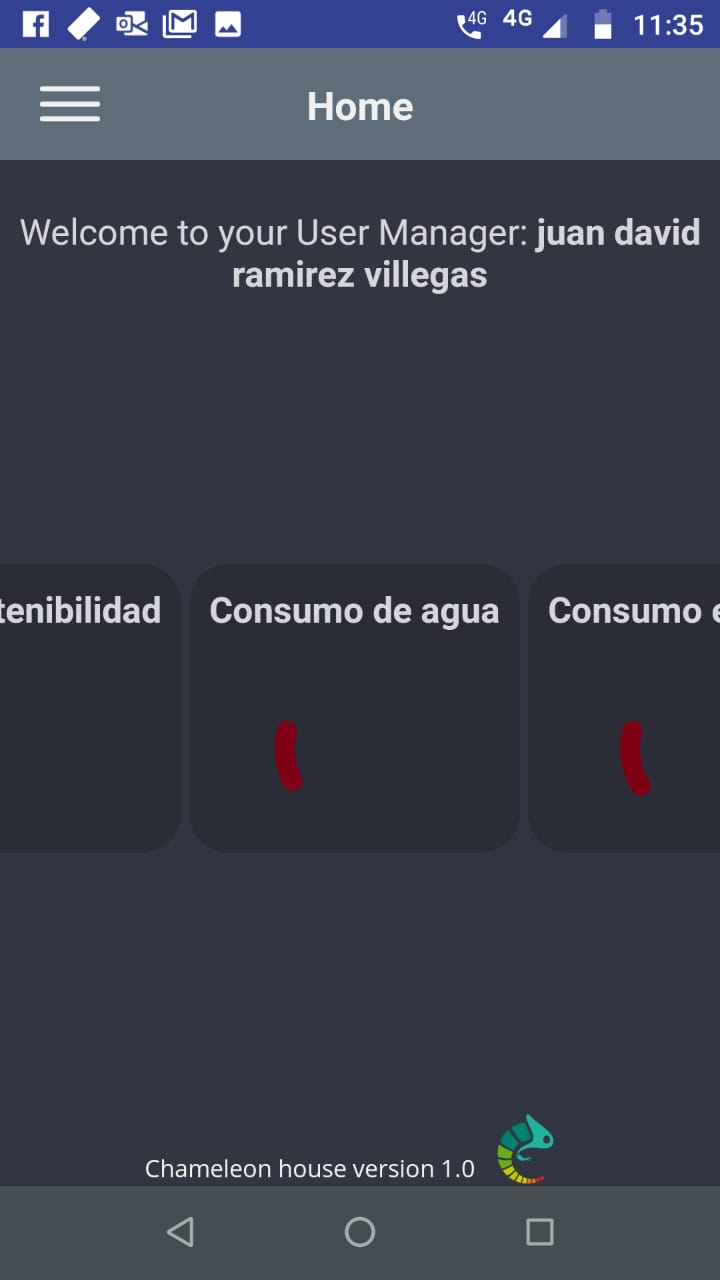
\includegraphics[width=5cm]{./figuras/mobile_home.jpeg}}
		\caption{Escena para la visualización del consumo histórico. Fuente: propia}
		\label{fig_14}
	\end{figure}
	\item  \textit{``La aplicación notificara al usuario cuando la factura este vencida:''} para este requerimiento se implementó una función adicional en el aplicativo en sitio, por ende, para esta versión de la aplicación no se desarrolló ningún componente relacionado con esta necesidad.
	
	\item \textit{``El usuario debe ser capaz de poder ver su impacto ambiental basado en datos cualitativos y cuantitativos:''} Teniendo en cuenta la figura \ref{fig_14} uno de los indicadores corresponde a un indicador de sostenibilidad que está basado en la huella de carbono del consumo de agua y el consumo eléctrico, pero el componente cualitativo no fue implementado para esta versión de la aplicación.
	
	\item \textit{``El sistema debe ser capaz de notificar las perdidas eléctricas y por consiguiente económicas de un mal uso de los horarios establecidos por defecto:''} Para implementar este requerimiento se desarrolló en el aplicativo en sitio la función de notificación automática.
	
\end{enumerate}


\subsection{Funciones adicionales}

En adición a los requerimientos funcionales se añadieron características a la conceptualización de diseño original, lo anterior, para mejorar el funcionamiento de la plataforma y la experiencia de usuario. Estas funciones se pueden ver a continuación:

\begin{enumerate}
	\item \textbf{Pantalla de control:} Teniendo en cuenta un diseño con el mayor control y administración de los actuadores y sensores conectados al sistema, para esta versión de la aplicación, se implementó una interfaz de control que se puede observar en la figura \ref{fig_16}, donde el usuario tiene la posibilidad de modificar la configuración horaria programada por defecto para el Solar Decathlon. Una vez el usuario altera el estado de los circuitos de la vivienda a través de la ventana, El sistema de agenda local se desactiva por 24 horas para darle la prioridad a lo que defina el usuario.
	
	\begin{figure}[htbp]
		\centerline{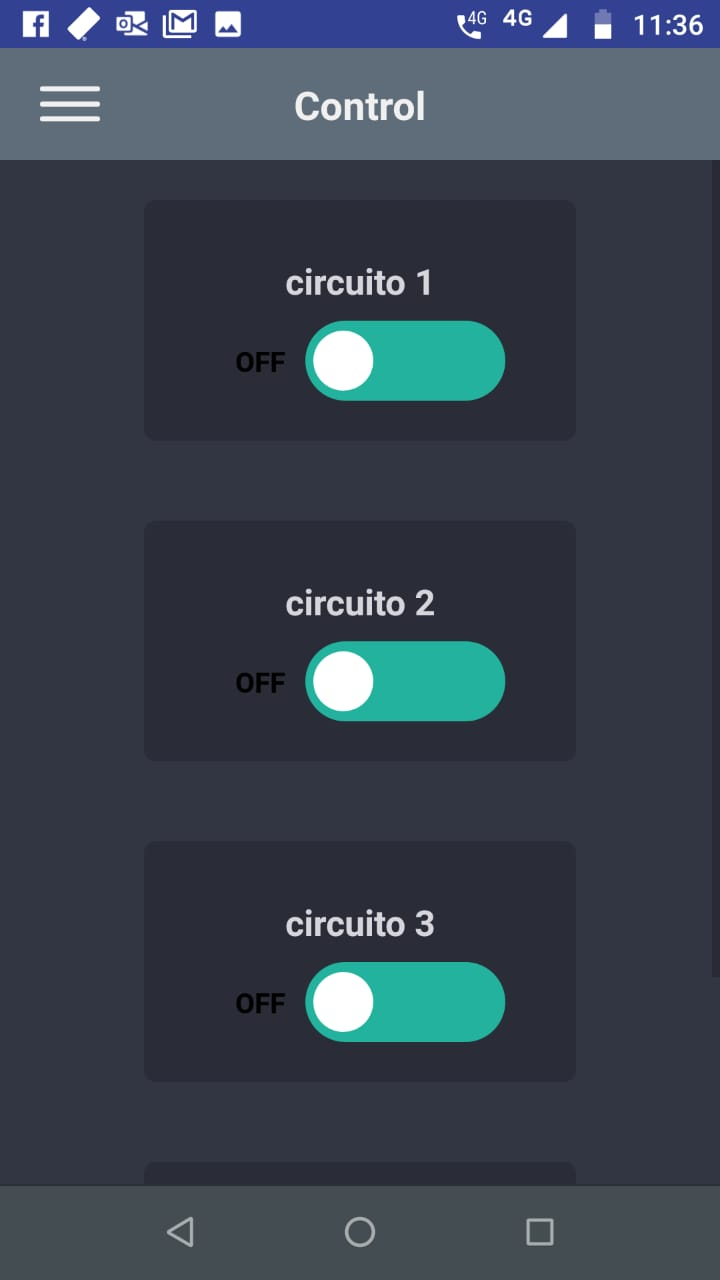
\includegraphics[width=5cm]{./figuras/mobile_control.jpeg}}
		\caption{Escena para el control de los circuitos de la vivienda. Fuente: propia}
		\label{fig_16}
	\end{figure}
	
	\item \textbf{Ventana de introducción:} Esta función es más un componente decorativo, la escena le da la bienvenida al usuario, mejora la experiencia de usuario y le da status a la interfaz. Figura \ref{fig_12}.
	
	\begin{figure}[htbp]
		\centerline{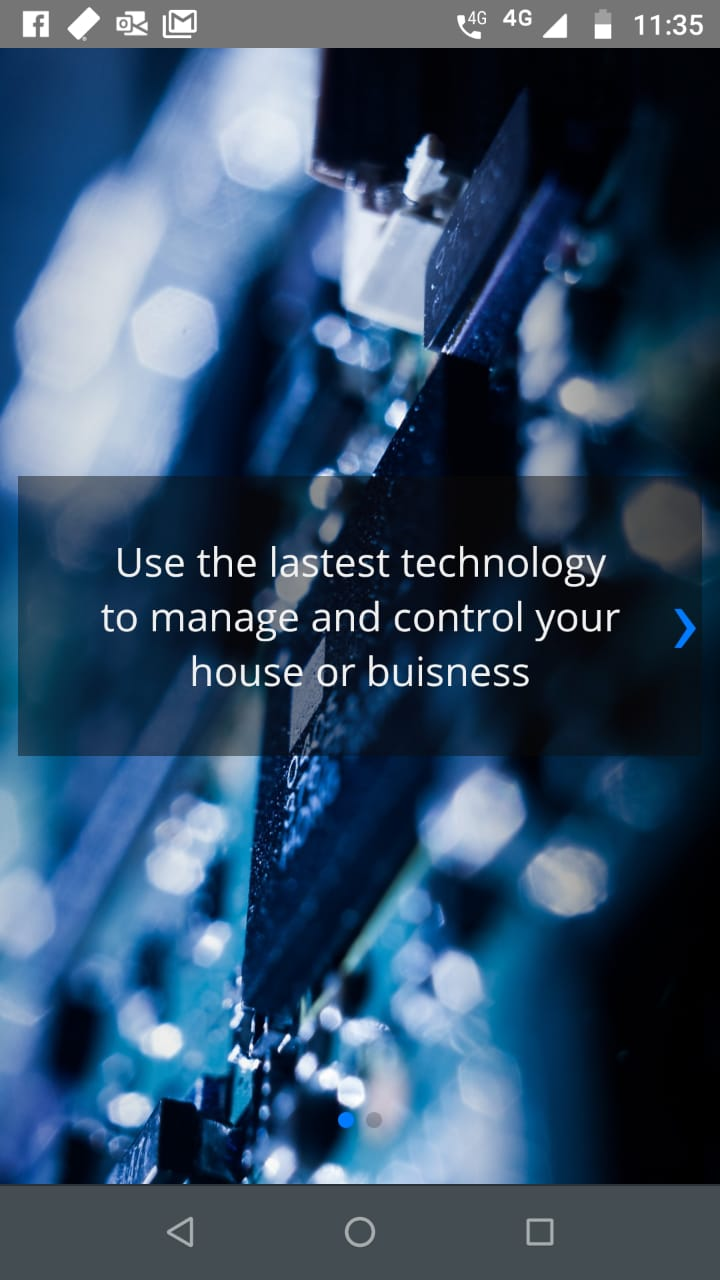
\includegraphics[width=5cm]{./figuras/mobile_intro1.jpeg}}
		\caption{Escena de bienvenida 1. Fuente: propia}
		\label{fig_12}
	\end{figure}
	
	\item \textbf{Servicio de autenticación:} Finalmente, se implementó un servicio de autenticación utilizando la api de Google, utilizando su api de autenticación se desarrolló la interfaz para obtener la información del usuario como: correo, numero de teléfono, nombre completo y una llave encriptada con la que la app puede re autenticar el usuario en caso de ser necesario tal como se ve en la figura \ref{fig_13}.
	
	\begin{figure}[htbp]
		\centerline{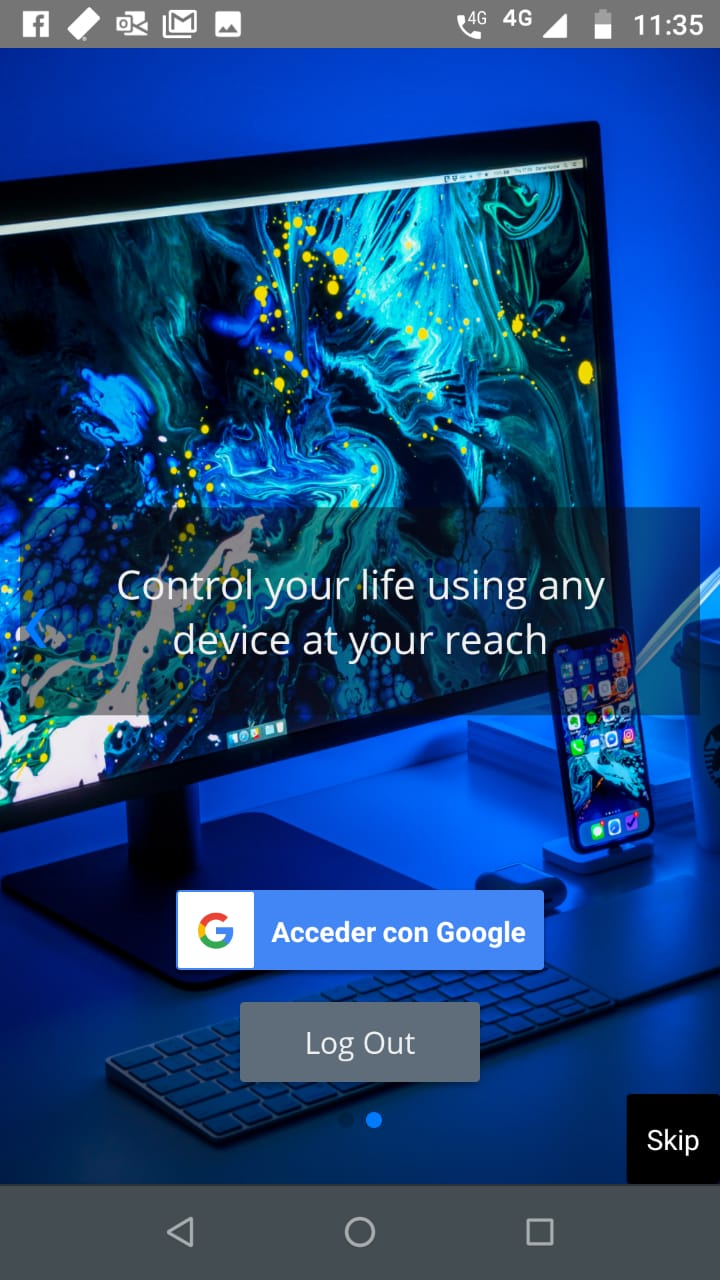
\includegraphics[width=5cm]{./figuras/mobile_intro2.jpeg}}
		\caption{Escena de inicio de sesión. Fuente: propia}
		\label{fig_13}
	\end{figure}	
\end{enumerate}

\subsection{Pruebas de concepto}
Para finalizar, debido a que el sistema desarrollado está constituido enteramente por software se decidió adicionar un componente de hardware para probar conceptualmente la capacidad de añadir cualquier sistema de medición o actuación.
\vspace{0.5cm}\\
Como dispositivo de medición se utilizó un medidor bifásico de la empresa Inelca con una interfaz de comunicación Rs485 \ref{32}. Utilizando esta interfaz y un conversor USB a Rs485 se logró comunicar la Raspberry con el medidor de Inelca.
\vspace{0.5cm}\\
\begin{figure}[htbp]
	\centerline{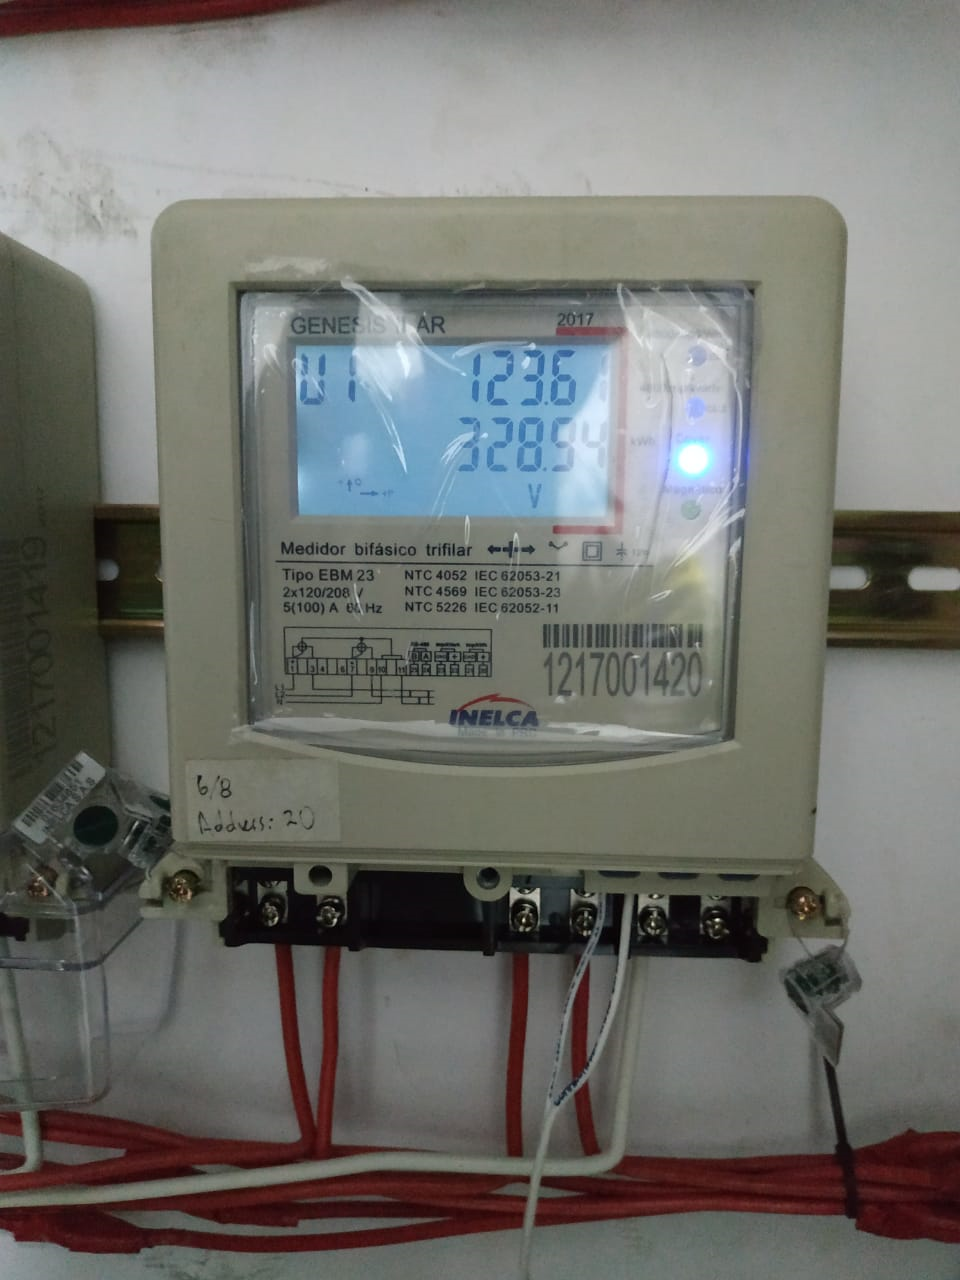
\includegraphics[width=5cm]{./figuras/concepto_1.png}}
	\caption{Dispositivo Inelca utilizado para la prueba de concepto. Fuente: propia}
	\label{fig_32}
\end{figure}

Para finalizar, se puso a prueba el sistema añadiendo la función de adquisición necesaria para obtener el valor del voltaje Rms del medidor a partir de una trama serial tipo modbus, tal como se observa en la figura \ref{fig_33}.

\begin{figure}[htbp]
	\centerline{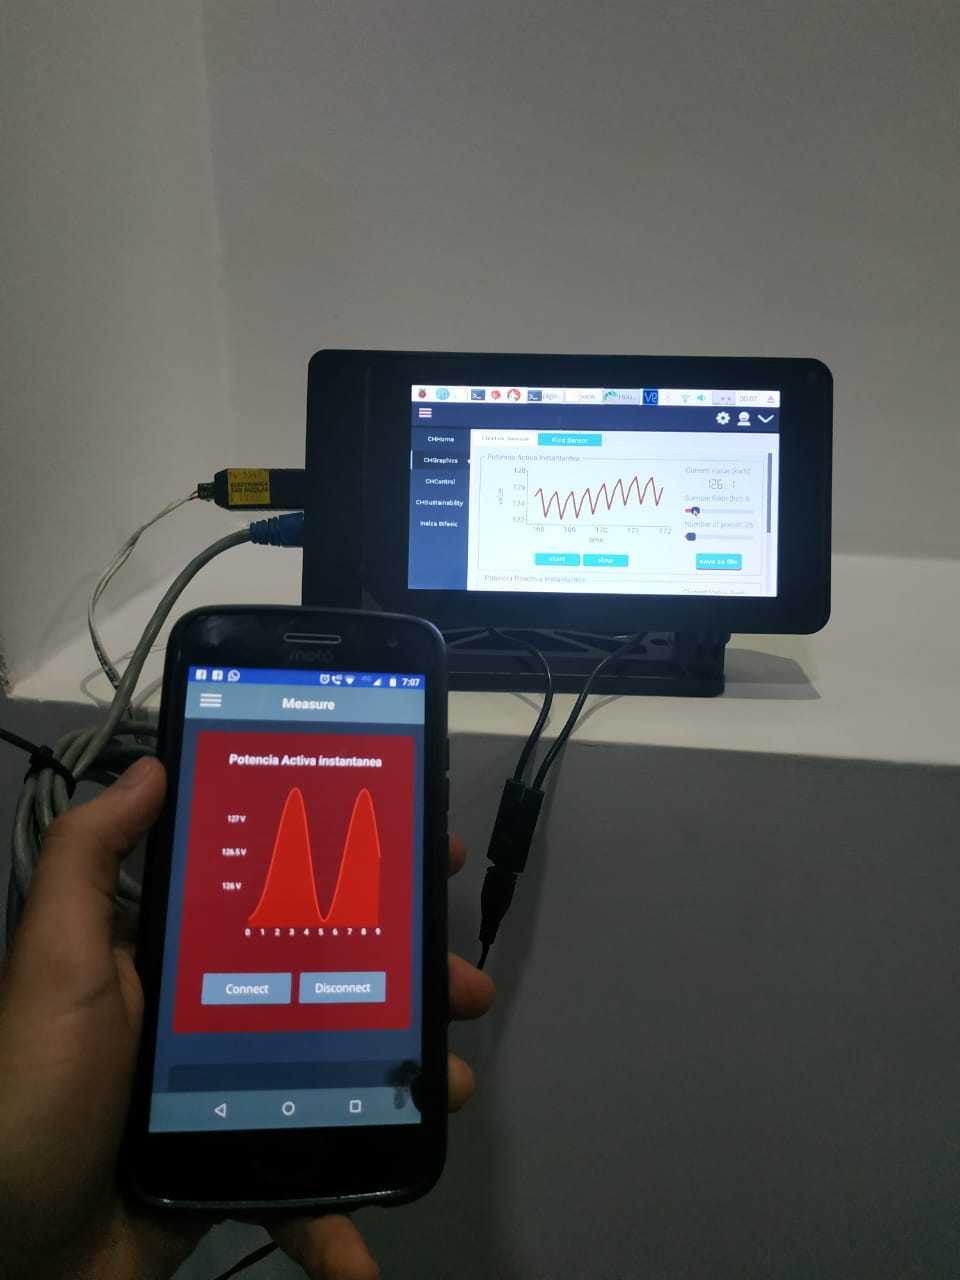
\includegraphics[width=5cm]{./figuras/concepto_2.png}}
	\caption{Prueba de concepto usando todos los sistemas. Fuente: propia}
	\label{fig_33}
\end{figure}




%-----------referencias------------------
%\section{Referencias}

\bibliography{bibliografia_anteproyecto_v1}
\nocite{*}
\bibliographystyle{apalike} %iee

%-------------------------------------
\end{document}

%********************
%%% FIN DEL DOCUMENTO!
%********************